\chapter{Identifying significant parameters combinations in complex
  models \label{ch:params}}


% \begin{abstract}
%   Detailed dynamical models can often be summarized in terms of only
%   a few components, reducing complexity and making exploration
%   easier and more insightful.  Pen-and-paper reduction is tedious
%   and impractical for most models, however it has the added benefit
%   of identifying parameter combinations that matter most.  Recently
%   developed frameworks computerizing model reduction leave the dual
%   aspect of effective parameter identification unaddressed,
%   relegating parameter space exploration subject to ineffective
%   sampling strategies.  Here, we lay the foundation for systematic
%   parameter reduction, rooting it in the same nonlinear data mining
%   techniques that powered model reduction in our earlier
%   equation-free framework.  Our ambition is to extend the
%   data-driven determination of effective variables by integrating
%   into it the discovery of effective model parameters.  This will
%   accelerate both dynamical simulations and parametric explorations,
%   allowing us to efficiently map out the behavior of complex models.

% \end{abstract}

The past decades have seen a steady fall in the cost of computation,
enabling systems to be studied using increasingly complex models.
Perceptron networks in the 1960's contained thousands of hidden units
\cite{nagy_neural_1991}, while modern neural nets are comprised of
billions \cite{hsu_biggest_2015}. Molecular dynamics simulations in
1957 entailed tens of hard-sphere particles \cite{alder_phase_1957};
today we model entire proteins and their folding dynamics
\cite{piana_atomic-level_2013}. And Lorenz's three-dimensional system
of equations describing atmospheric convection in 1963
\cite{lorenz_deterministic_1963} led to modern large eddy simulations
run across multiple computing clusters \cite{ghosal_dynamic_1995}. In
all cases, the improvement in precision afforded by increased model
complexity is matched by an increased number of model parameters.

Highly parameterized models may aid accuracy, but the effect of each
individual parameter on the overall model output is often difficult to
ascertain. Indeed, it has been well-document that a wide array of
systems contain particular hidden parameters that appear to have no
influence on the model's predictions
\cite{gutenkunst_extracting_2007}. These have been termed ``sloppy
parameters'', and their presence seems ubiquitous in contemporary
systems \cite{gutenkunst_universally_2007}. This is problematic as not
only do sloppy parameters obfuscate the inputs that actually
matter, but they also lead to slow convergence of model-fitting
algorithms \cite{transtrum_geometry_2011}.

Several approaches have been suggested to combat this
over-parameterization. Some, such as the Manifold Boundary
Approximation Method ultimately rely on deriving by hand a reduced
model \cite{transtrum_model_2014}. Others, such as Active Subspaces
make assumptions about linearity that may not hold in practical
settings \cite{constantine_active_2015}. Here, we present a
data-driven approach to parameter reduction that is flexible enough to
handle nonlinear systems. This is accomplished through Diffusion Maps
(DMAPS), an established manifold learning technique that we adapt to
this context \cite{coifman_diffusion_2006}. We begin with a
description of our formulation of the problem, and then present a
simple example that clearly shows the consequences of sloppiness,
while also providing some intuition as to how it emerges.

Our overall approach is motivated by the work in
\cite{transtrum_geometry_2011}. We consider a model to consist of a
vector of parameters $\theta \in \mathbb{R}^k$ and a function mapping
these inputs to a model response (or model output) in $\mathbb{R}^n$,
$f: \mathbb{R}^k \rightarrow \mathbb{R}^n$. Sloppiness would reveal
itself as regions of parameter space, $\Omega_S \in \mathbb{R}^k$ in
which the model reponse remains nearly constant:
$f(\theta_i) \approx f(\theta_j)\; \theta_i, \theta_j \in
\Omega_S$. We will also denote distances in parameter space as
$\delta(\theta_i, \theta_j) = \| f(\theta_i) - f(\theta_j)\|_2$, that
is, the Euclidean distance between the resulting model responses. To
provide a concrete example, consider a model with parameters $p_1$ and
$p_2$, and model output
$f(p_1, p_2) = (p_1 p_2 , \ln(p_1) + \ln(p_2) , (p_1 p_2)^2)$. Then
$\theta = (p_1, p_2) \in \mathbb{R}^2$ and $f: \R^2 \rightarrow
\R^3$. It is clear from the expression for $f$ that the model response
depends only on the overall product $p_1 p_2$, and not on $p_1$ and
$p_2$ independently. To make it explicit, set $p_{eff} = p_1 p_2$ and
rewrite $f$ as $(p_{eff}, \ln(p_{eff}), p_{eff}^2)$. Thus, although we
have chosen to include both $p_1$ and $p_2$ as independent parameters
in our original model, only the value of $p_{eff}$ is significant. Also note
that if we only had access to a black-box function evaluator, it would
be non-trivial to determine the existence of $p_{eff}$ at all.

This model is illustrated in Figure~\ref{fig:non-id}, where curves of
constant color denote sets of constant model response. If we had
sampled data corresponding to true parameter values of
$p_1^* = p_2^* = 1$, Figure~\ref{fig:non-id} also reveals how
sloppiness affects optimization routines trying to fit such
data. Convergence is permitted along entire bands of parameter space
instead of at a single point. The inset shows $\delta$-contours of a
slightly perturbed system in which both $p_1$ and $p_2$ influence $f$;
however, certain directions, namely along the diagonal, still affect
model output more strongly than others. In addition, optimization
routines will still converge to disparate points in the plane: the
model remains sloppy.

Our goal, then, is to extract the appropriate, intrinsic
parameterization of the model using only input-output data. As we
shall see, this parameterization may vary across input space regimes.
We will show how this variation can be associated with the traditional
notions of regular and singular perturbations in explicit models when
the number of effective parameters changes.


\begin{figure}
  \centerline{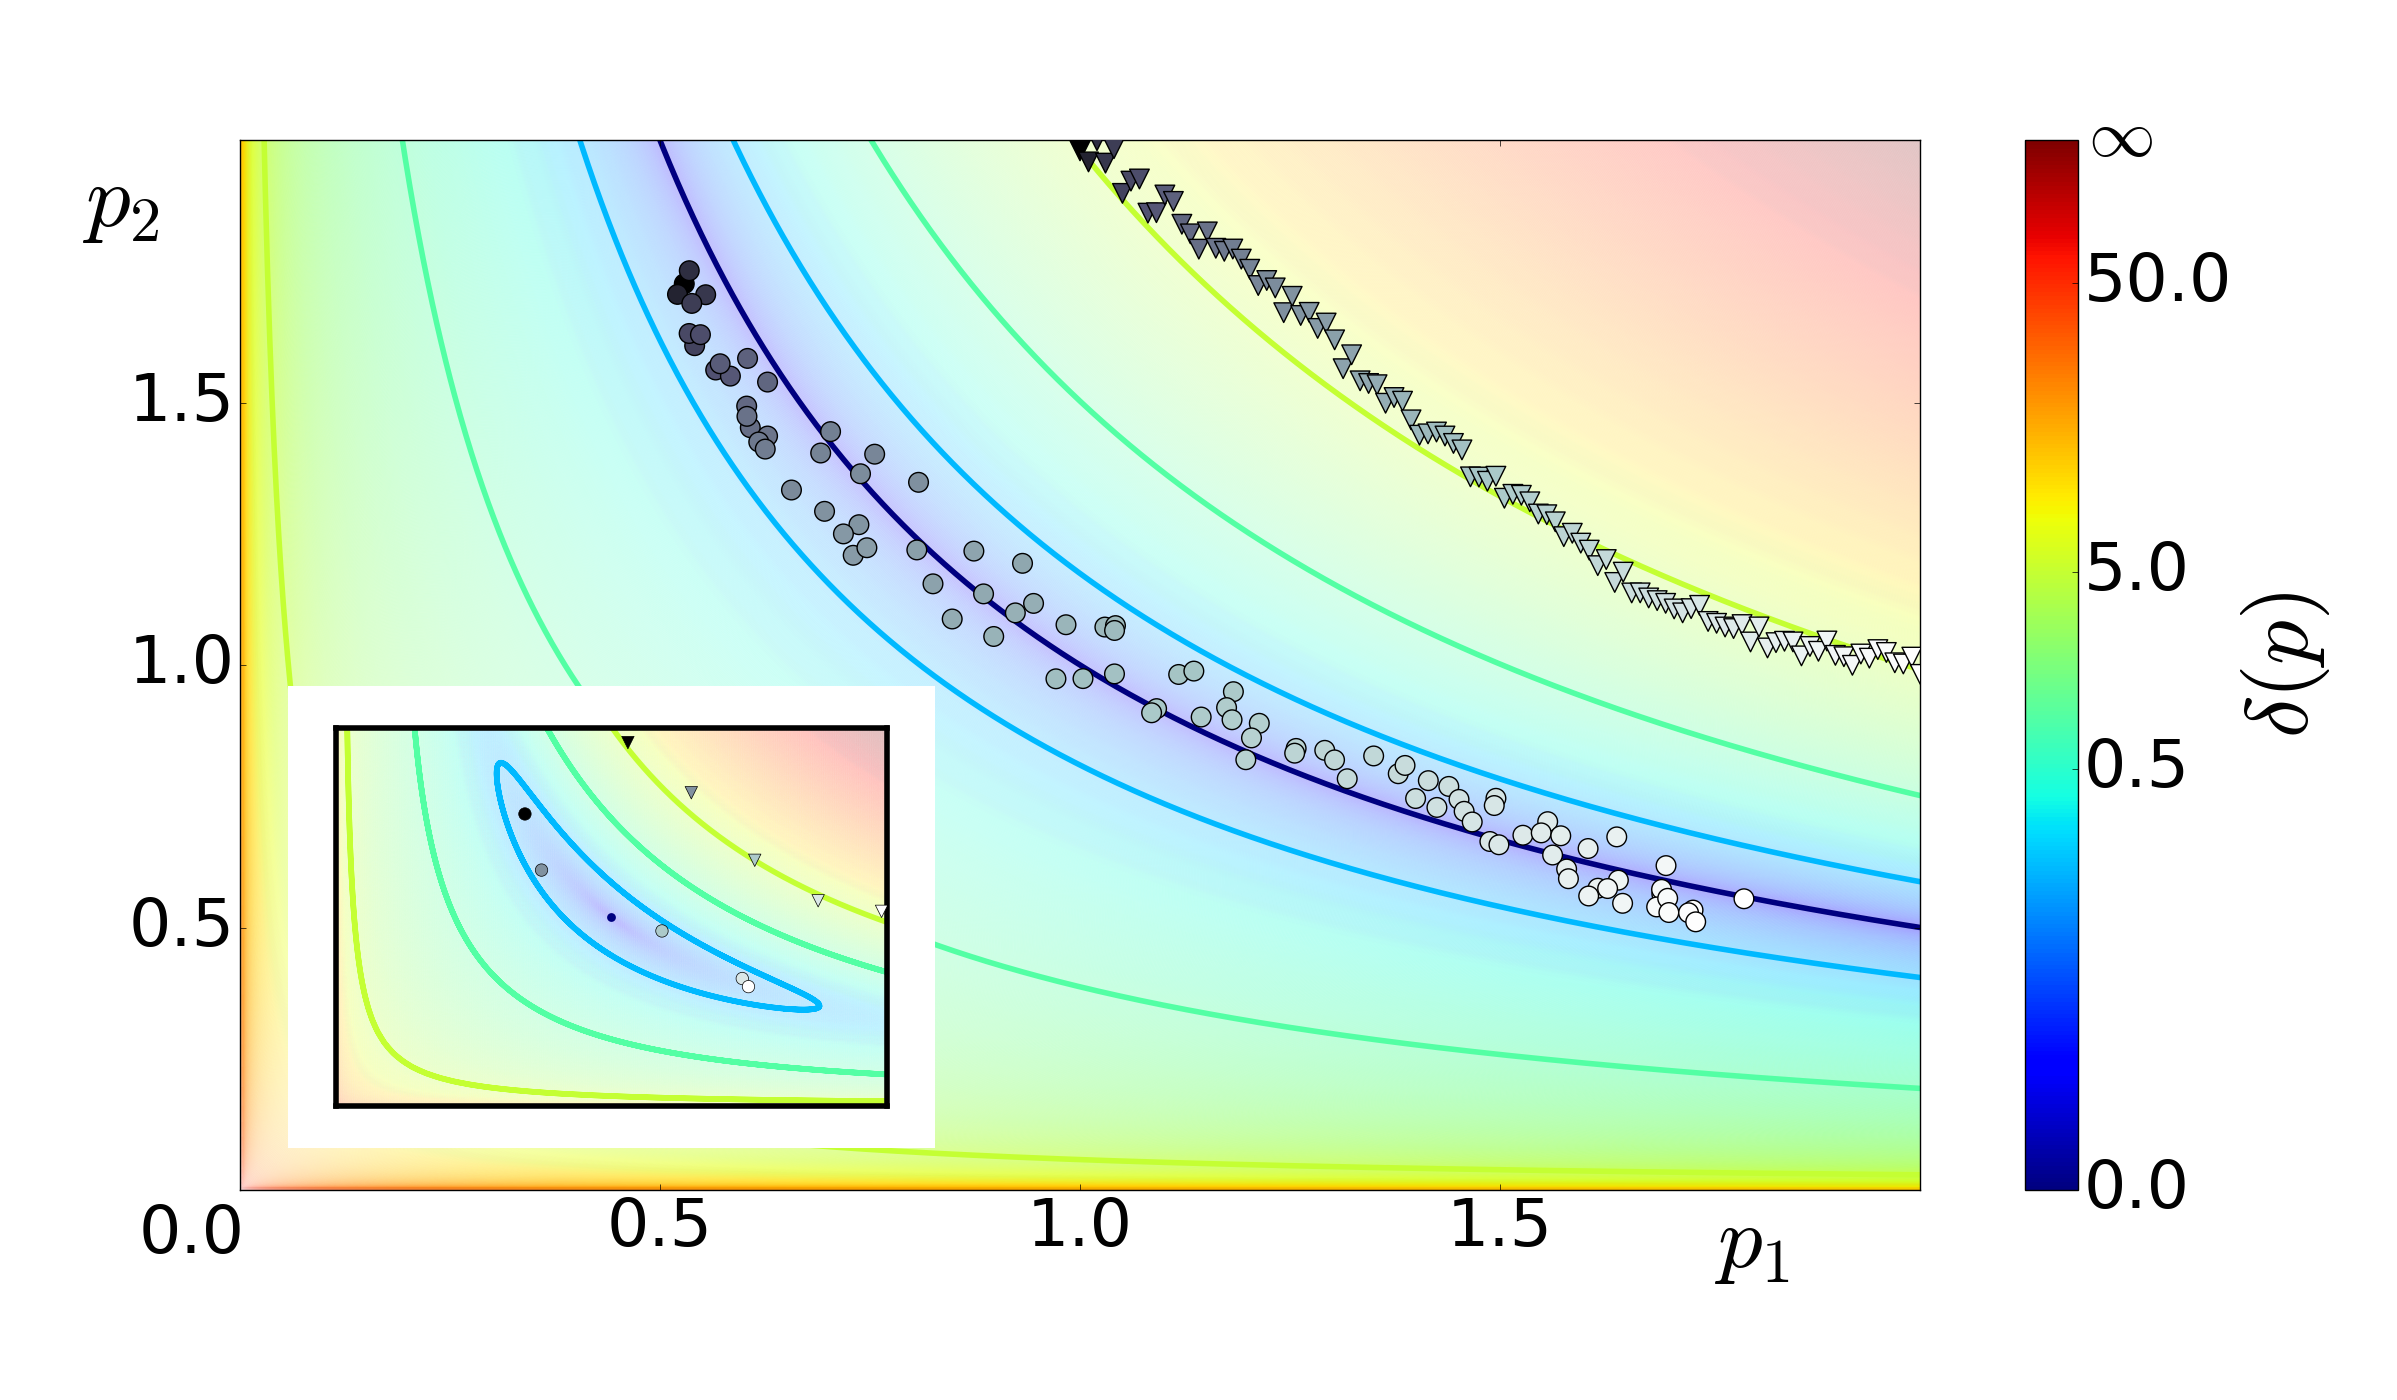
\includegraphics[width=1.0\linewidth]{p2-p1-delta}}
  \caption[Illustration of effects of sloppiness on
  optimization]{Coloring the $(p_1, p_2)$ plane by $\delta$ for
    $f(\theta) = (p_1 p_2 , \ln(p_1) + \ln(p_2) , (p_1 p_2)^2)$ (main
    figure) and the perturbed $g(p1, p2) = f(p_1, p_2) +
    \left(2*\epsilon*(p1 - p2), 0, 0\right)$ with $\epsilon = 0.2$
    (inset). $\delta$ values are calculated with respect to the base
    parameters $p^* = (1, 1)$: $\delta(p_1, p_2) = \| f(p_1, p_2) -
    f(p_1^*, p_2^*)\|$. Also shown are a range of initial and final values of
    a gradient descent algorithm. For $f$, convergence can occur
    anywhere along the infinite band for which $\delta$ is less than
    the accepted tolerance. For $g$, convergence is confined to
    bounded but stretched regions in the plane.
    \label{fig:non-id} }
\end{figure}



\section{Example from chemical kinetics} \label{sec:rr}

We now examine a system of chemical reactions in which an effective
parameter again emerges, and show how we can detect this in a
data-driven manner. The three-species system is

\begin{align}
  A
  \xrightleftharpoons[k_{-1}]{k_1}
  B
  \xrightarrow[]{k_2}
  C
  \label{mech:abc}
\end{align}

Under mass action kinetics, the concentration of the end product is
given by the analytical expression
% 
\begin{align}
  C(t|\theta)
  =
  A_0
  \left(
  \frac{k_1 k_2}{\alpha \beta}
  +
  \frac{k_1 k_2}{\alpha(\alpha - \beta)}
  e^{-\alpha t}
  -
  \frac{k_1 k_2}{\beta(\alpha - \beta)}
  e^{-\beta t}
  \right)
  \label{eq:cfull}
\end{align}
% 
where $(A_0,B_0,C_0)$ are the fixed constituent concentrations at time
zero and $\alpha,\beta$ depend on $\theta=(k_{-1},k_1,k_2)$; see
Appendix~\ref{app:abc} for the derivation. In the parameter regime
$k_1 k_2 \ll (k_1 + k_{-1} + k_2)^2$, \eqref{eq:cfull} is well
approximated by
% 
\begin{align}
  C_{eff}(t|\theta)
  =
  A_0
  \left(
  1 - e^{-k_{eff} t}
  \right) ,
  \quad
  k_{eff}
  =
  \frac{k_1 k_2}{k_{-1} + k_1 + k_2} .
  \label{eq:abc-qssa}
\end{align}
% 
Note that this approximate solution extends to a larger parameter
range the quasi-steady state approximation (QSSA)
$C_\mathrm{QSSA}(t|\theta) = A_0 (1 - e^{-k_\mathrm{QSSA} t})$, valid
for $k_1 \ll k_{-1} + k_2$ with
$k_\mathrm{QSSA}=k_1 k_2/(k_{-1} + k_2)$.  Plainly, this approximate
solution represents an effective reduction of parameter space down to
the single parameter $k_{eff}$, the levels sets of which foliate
parameter space as in Fig.~\ref{fig:abc-ill}.

To verify that $C(t)$ remains roughly constant on these level sets, we
choose reference parameter settings $\theta^*$ in the regime
identified above, fix sampling times $t_1,\ldots,t_N$, set the model
response to $f(\theta)=( C(t_1|\theta) , \ldots , C(t_N|\theta) )$,
sample log-parameter space uniformly, and record the squared Euclidean
distance $\delta(\theta) = \| f(\theta) - f(\theta^*) \|^2$ for each
sampled $\theta$.  Figure~\ref{fig:abc-keff} shows the results colored
by $k_{eff}$. We only retained parameter combinations with
$\delta(\theta) < 10^{-6}$ to aid in visualization. As expected, the
level sets of constant $\delta$ align with those of the effective
parameter, so this automated sampling process effectively reveals
sheets of different $k_{eff}$ values without recourse to an analytic
expression.

\begin{figure}[!htp]
  \centering
  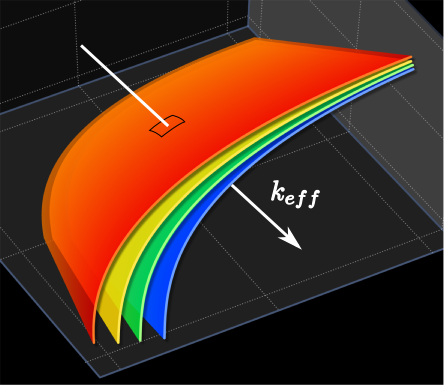
\includegraphics[width=0.4\textwidth]{keff-illustration}
  \caption[Illustration of level sets of the effective parameter in a
  model of chemical kinetics]{Illustration of level sets of $k_{eff}$
    in parameter space. \label{fig:abc-ill}}
\end{figure}


\begin{figure}[ht!]
  \centering
  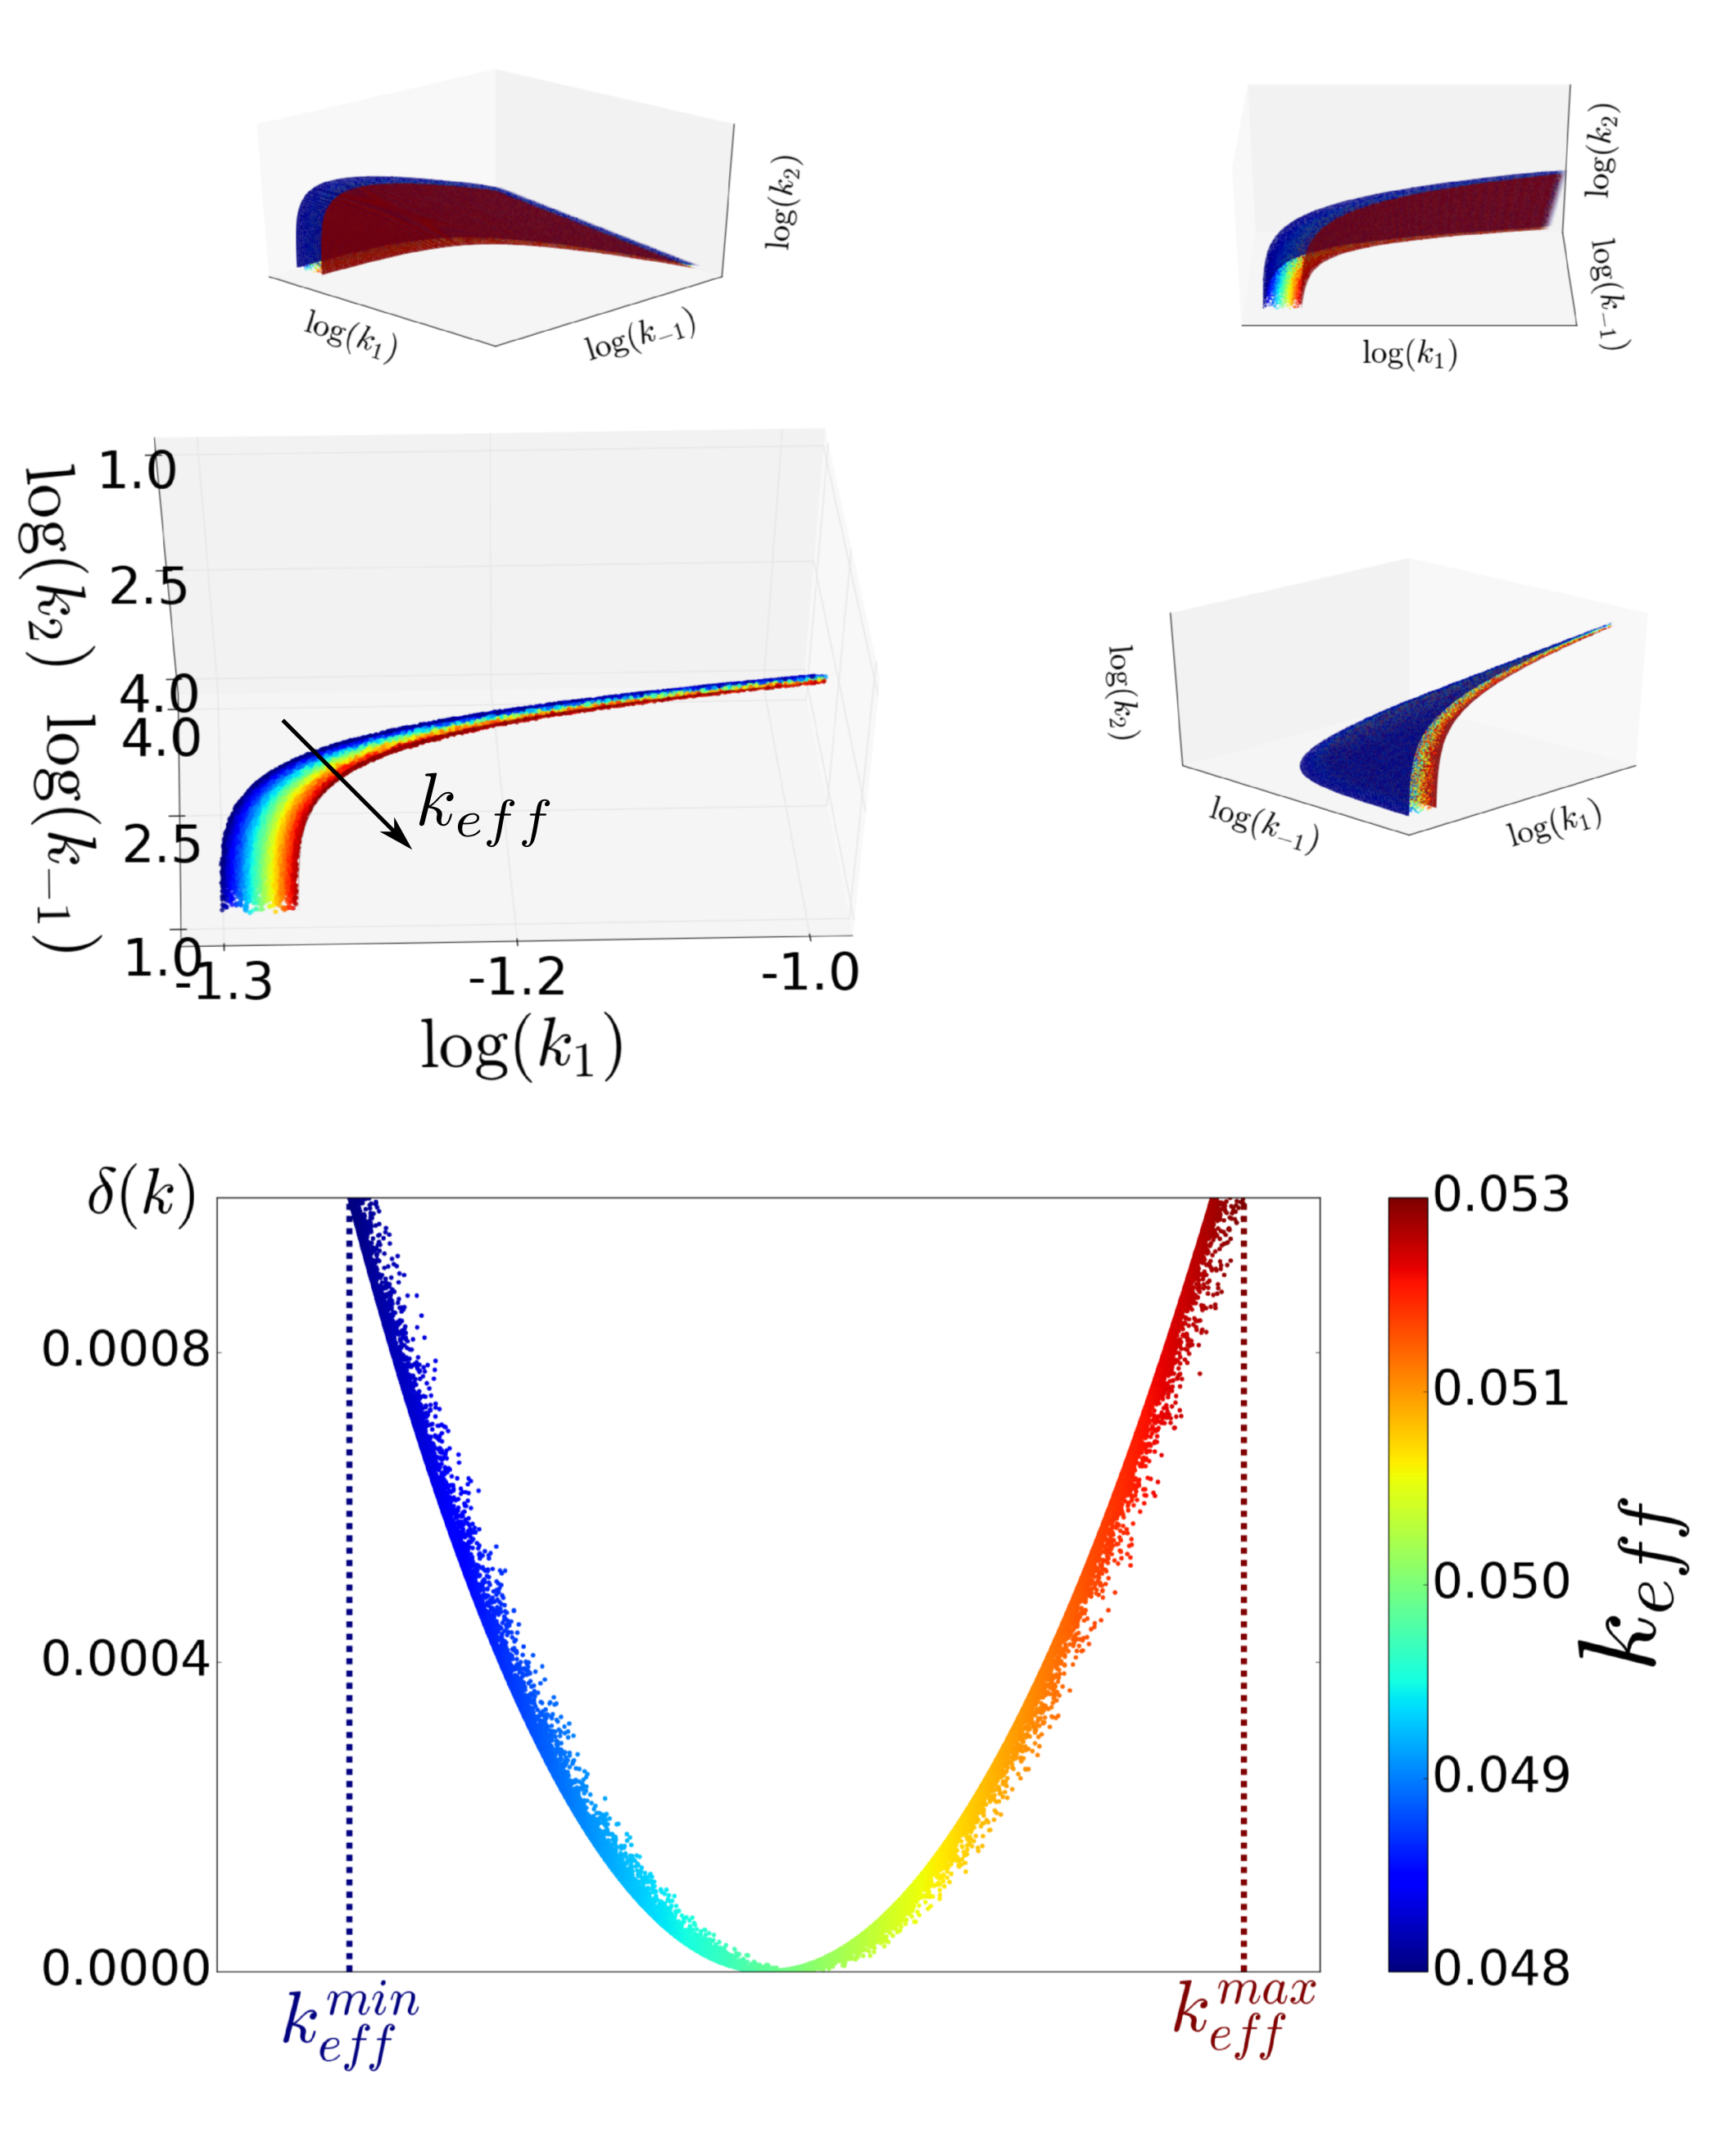
\includegraphics[width=0.9\textwidth]{keffs-delta-keff-vertical}
  \caption[Quantitative three-dimensional views of level sets of the
  effective parameter in a model of chemical kinetics]{(top) Region of
    parameter space lying within large value of $\delta = 10^{-3}$,
    colored by $k_{eff}$. Smaller rotations show three-dimensional
    structure. (bottom) Plot of $\delta$ vs $k_{eff}$ over the dataset
    showing that $\delta(k_1, k_{-1}, k_2) = \delta(k_{eff})$ as
    expected from the reduced reaction kinetics. \label{fig:abc-keff}}
\end{figure}


\begin{figure}[!htp]
  \centering
  \begin{tabular}{cc}
    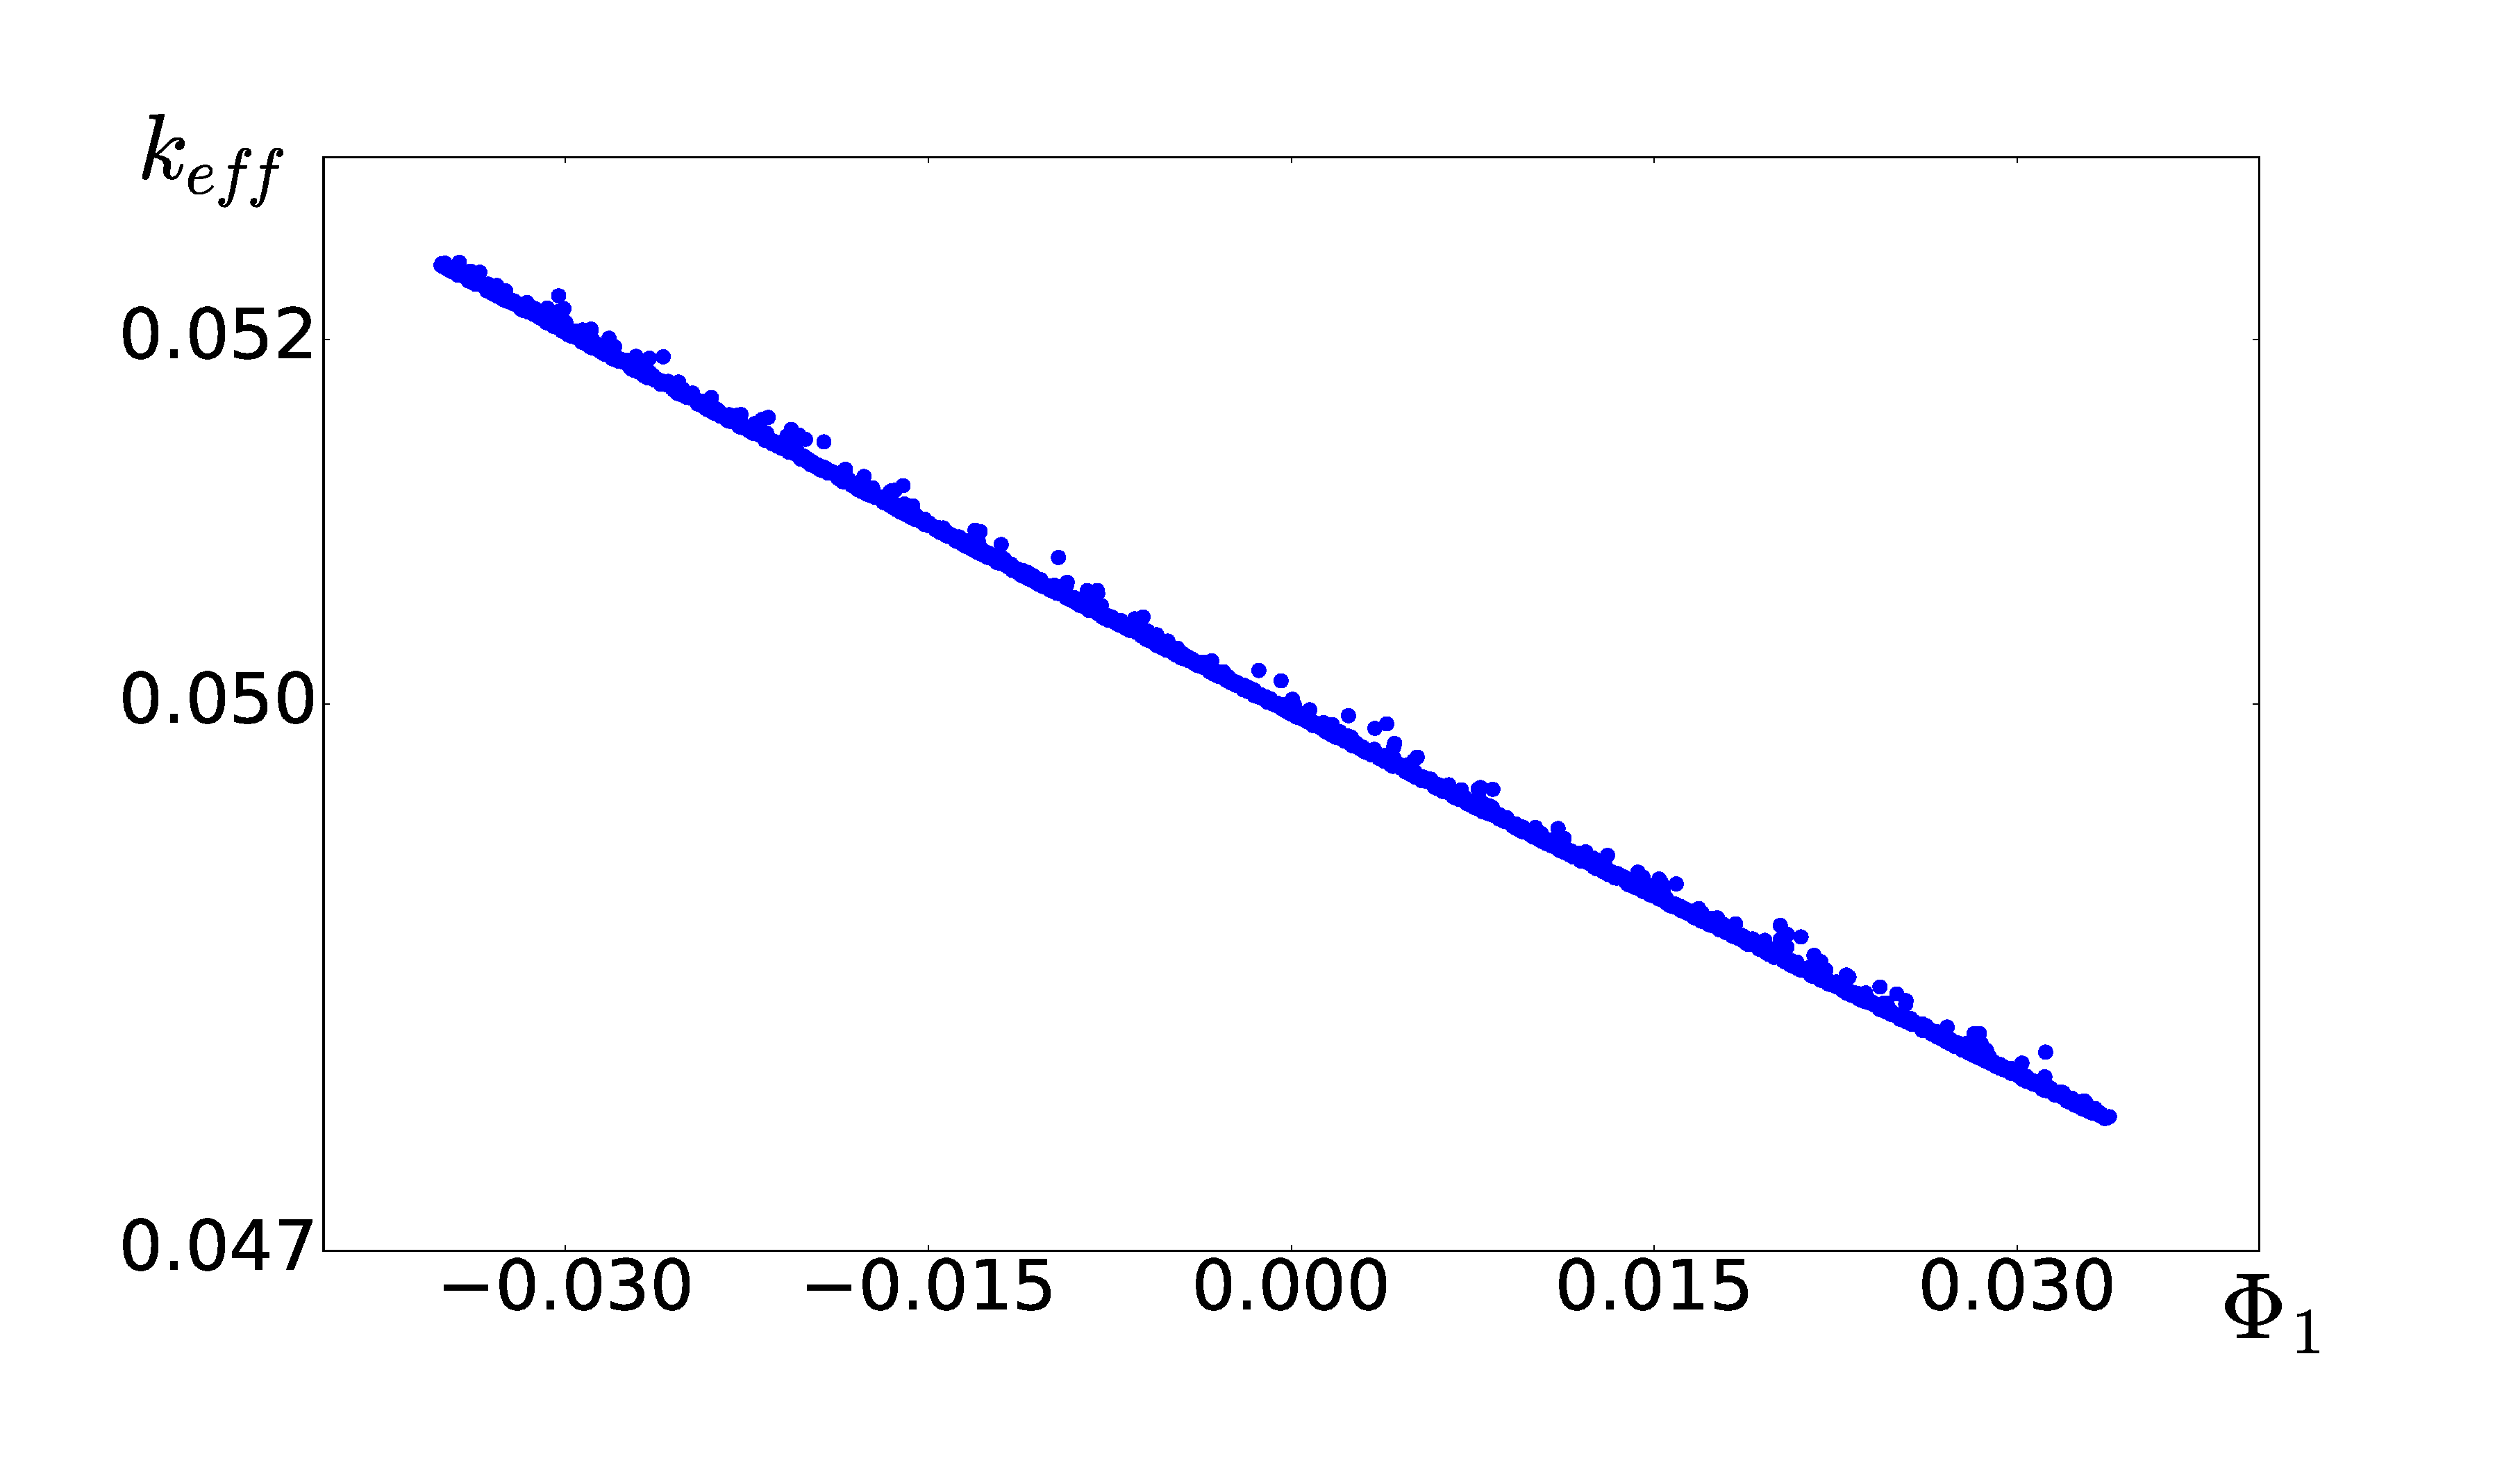
\includegraphics[width=0.45\textwidth]{keff-phi1} &
                                                        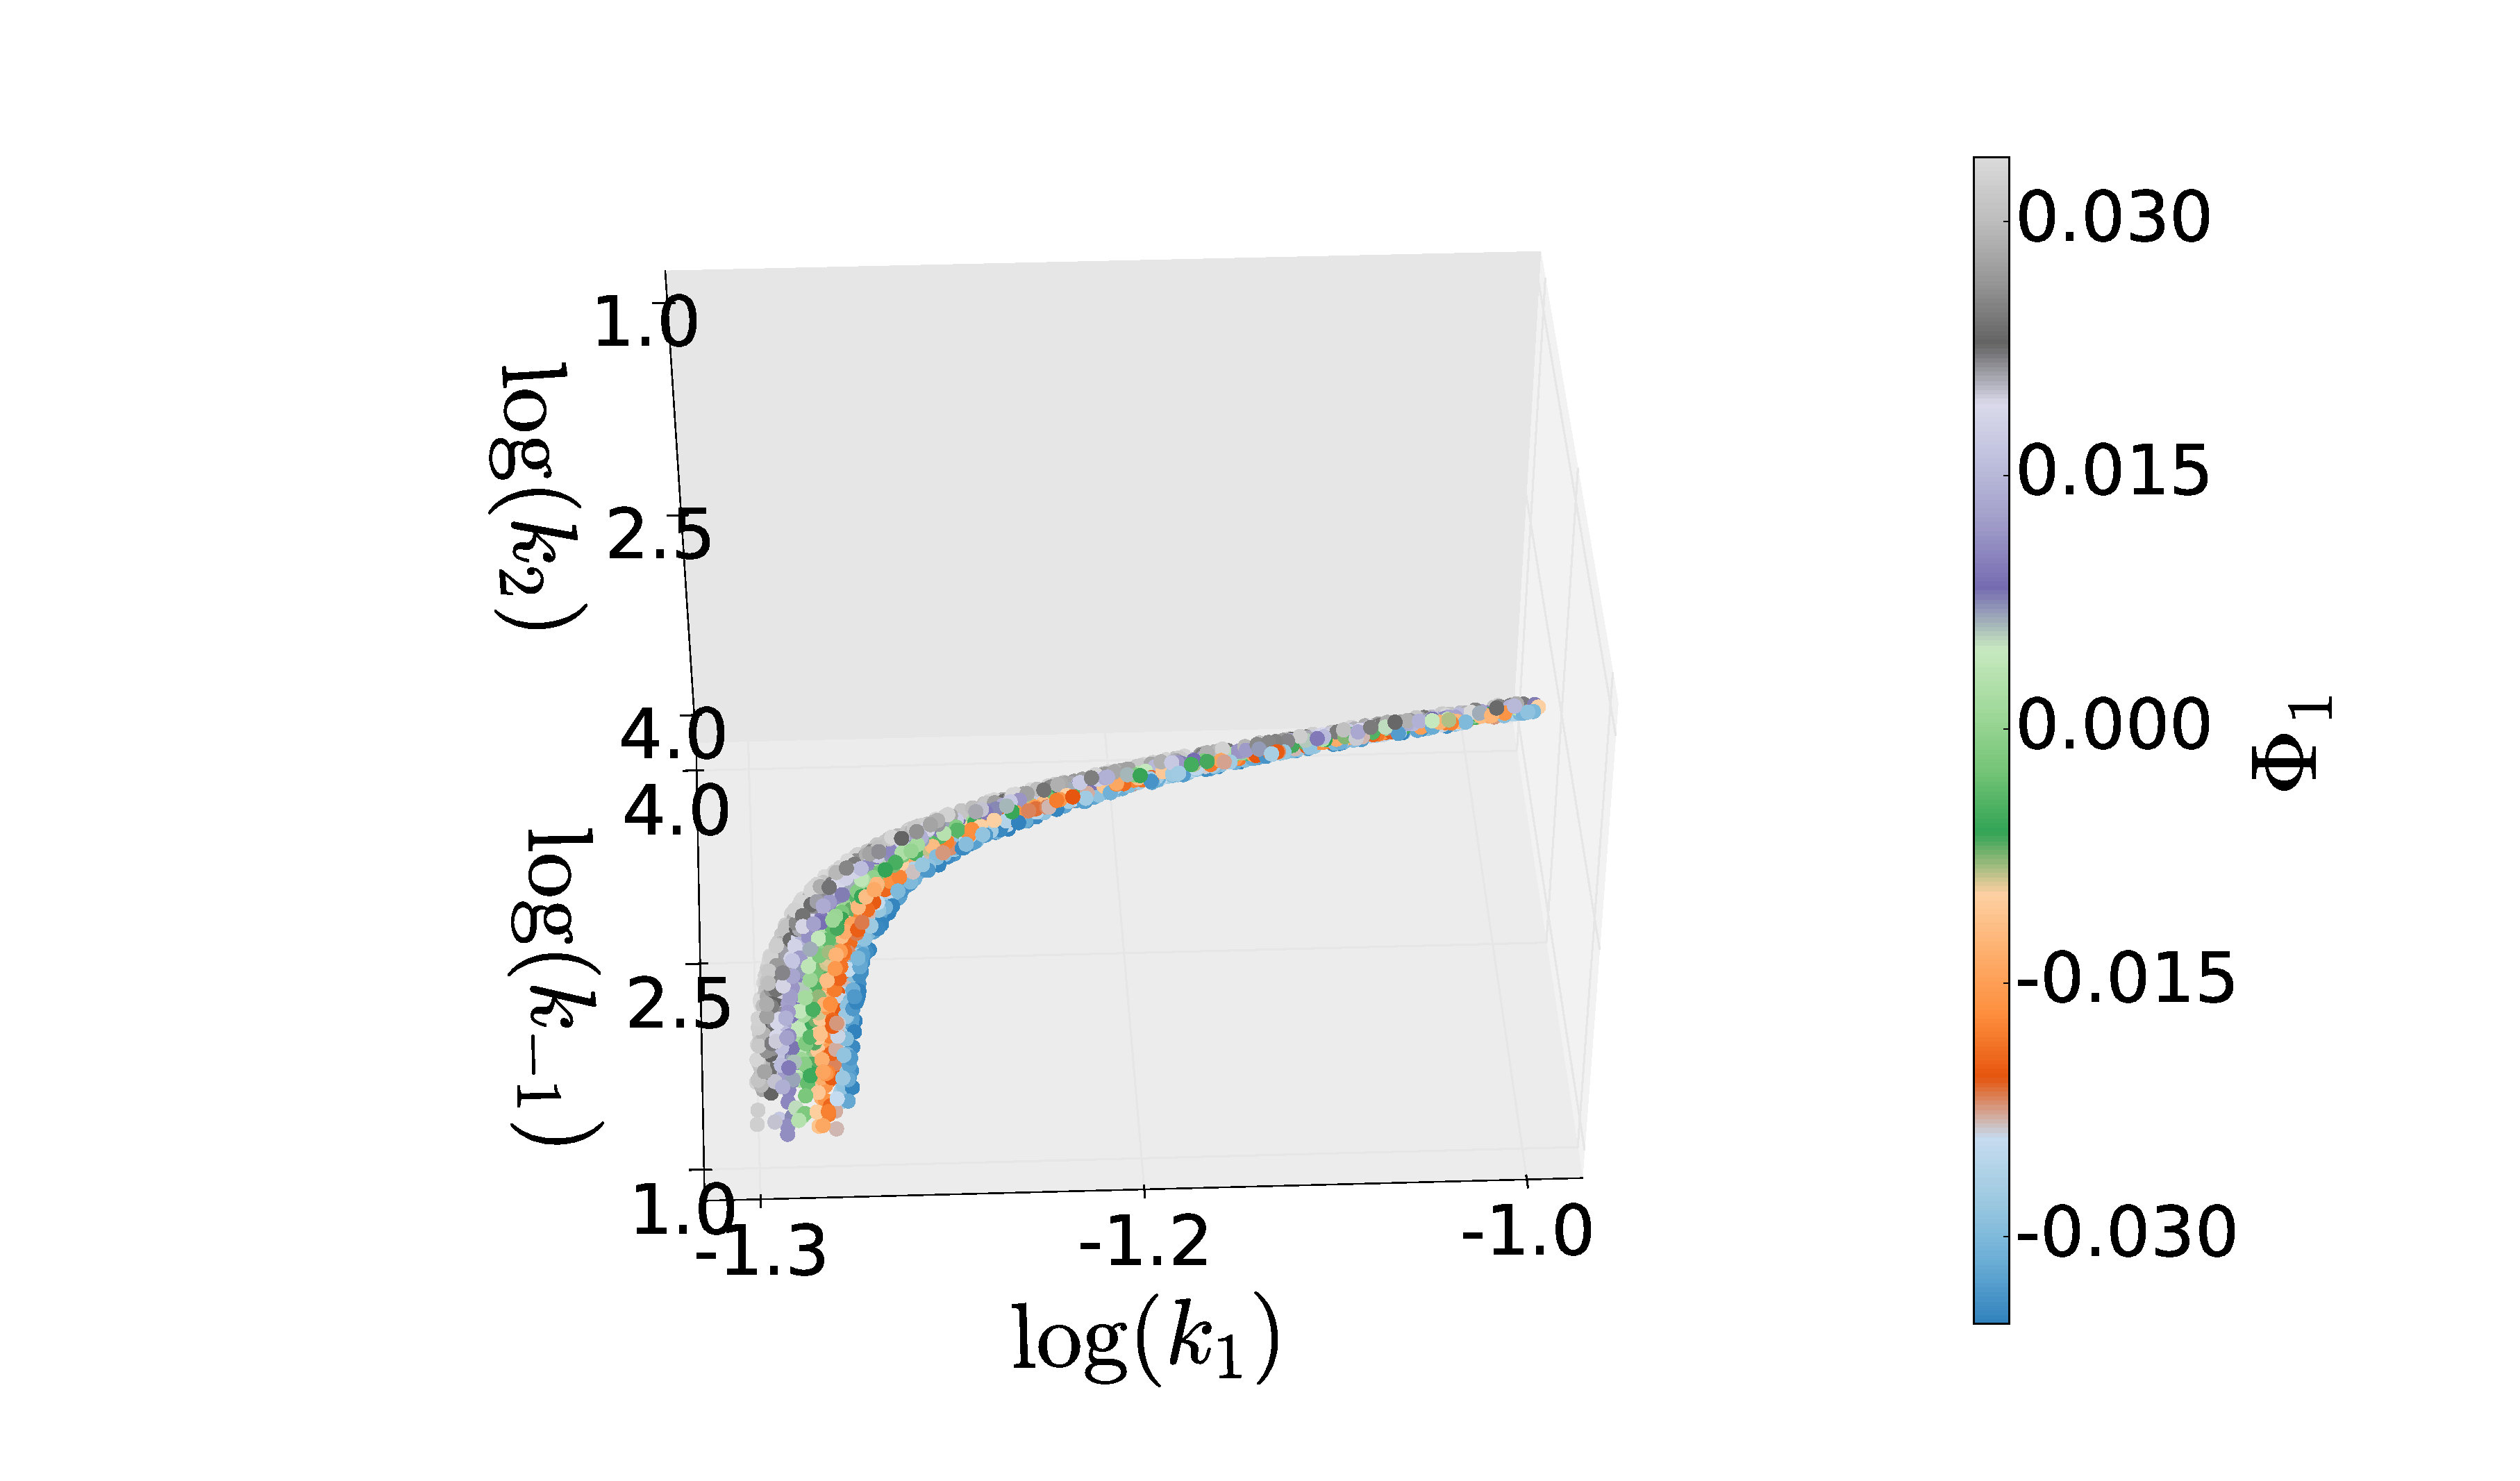
\includegraphics[width=0.5\textwidth]{k2-kinv-k1-phi1}\\
    (a) & (b)
  \end{tabular}
  \caption[DMAPS results for simple kinetic model]{(a) Coloring parameter space by $\phi_1$, showing that
    $\phi_1$ captures the effective parameter in this system; (b)
    $k_{eff}$ plotted against $\phi_1$ showing that the first DMAPS
    eigenvector parameterizes the significant, nonlinear parameter
    combination hidden in our model. \label{fig:abc-dmaps}}
\end{figure}


With this data in hand, we turn to a description of our modified
DMAPS algorithm. Details of the basic algorithm can be found in
Section~\ref{sec:dmaps}. In brief, given a collection of parameter
values ${\theta_i}_{i=1}^N$, we define our DMAPS kernel as

\begin{align}
  k(\theta_i, \theta_j) = \exp \left(-\frac{\|f(\theta_i) -
  f(\theta_j)\|^2}{\epsilon^2} \right)
  \label{eq:dmaps-mm}
\end{align}

The key point is that while the data in Figure~\ref{fig:abc-keff}
obviously represent a sample of parameter space, they simultaneously
sample the model response space through $f(\theta)$. Considering the
structure of this space, we can understand that all of the points
lying on a surface of constant $k_{eff}$ will be mapped to
approximately the same point in model response space: they share the
same output concentration trajectory as seen in
Equation~\ref{eq:abc-qssa}. Only changes in $k_{eff}$ affect the model
output, and thus our data will lie along a one-dimensional curve in
model response space, parameterized by $k_{eff}$. Therefore, if we
apply DMAPS to the model response data, the first eigenvector $\phi_1$
will yield a parameterization of this curve and we expect $k_{eff}$
and $\phi_1$ to be in one-to-one correspondence. This is precisely
what Figures~\ref{fig:abc-dmaps} shows. DMAPS has, in effect,
uncovered the effective parameter hidden in the system using only
parameter and model response data. We will now investigate how
sloppiness can arise in singularly- and regularly-perturbed systems,
and we will see that DMAPS is able to provide a more uniformly
significant reparameterization.


\section{Regular perturbation}

Let us now consider the differential equation
%
\begin{equation}
  \frac{dy}{dt} = \epsilon y^3 - y
  \quad
  y(0) = y_0 ,
  \label{1D-model-regpert}
\end{equation}
%
with $\theta = (y_0, \epsilon)$ and
$f(\theta) = \left(y(t_1), y(t_2), \dots, y(t_n) \right)$.

Unlike the previous two examples, there is no effective parameter
hidden in this system; however, our parameters affect the model output
very differently depending on their specific values. To see why this
is, consider what happens as $\eps \rightarrow 0$. The system becomes
regularly perturbed, and converges to the simpler
$\frac{dy}{dt} = -y$. Note that in this limit, $\eps$ has no influence
on the model response, and $y_0$ becomes the only significant
parameter. Again, considering the implications for the model manifold,
it is clear that for small values of $\eps$, our response will form a
one dimensional curve parameterized by $y_0$. At larger values, both
$\eps$ and $y_0$ are significant, and the manifold is
two-dimensional. Figure~\ref{fig:regpert} (a) depicts the model
manifold colored by $\eps$, and we see exactly this behavior. The red
portion of the surface, corresponding to larger $\eps$, is
two-dimensional, while the blue, with small $\eps$, is contained in a
single line at the edge of the surface. Sampling this manifold, as
detailed in Appendix~\ref{app:regpert}, and applying DMAPS with the
kernel presented in Equation~\ref{eq:dmaps-mm} yields the same
information directly from data. Figure~\ref{fig:regpert} (b) shows the
$(\eps, y_0)$ parameter plane colored by $\phi_1$. At larger values of
$\eps$ the colors vary without any significant trend as this region is
two-dimensional. However, at small $\eps$, the colors flatten out
horizontally: $\phi_1$ is constant along lines of constant
$y_0$. DMAPS captures the fact that only one direction in parameter
space is relevant in the regularly perturbed regime. To continue along
this line in a slightly more complicated scenario, our next system
will be singularly perturbed.

\begin{figure}[ht!]
  \centering
  \begin{tabular}{cc}
    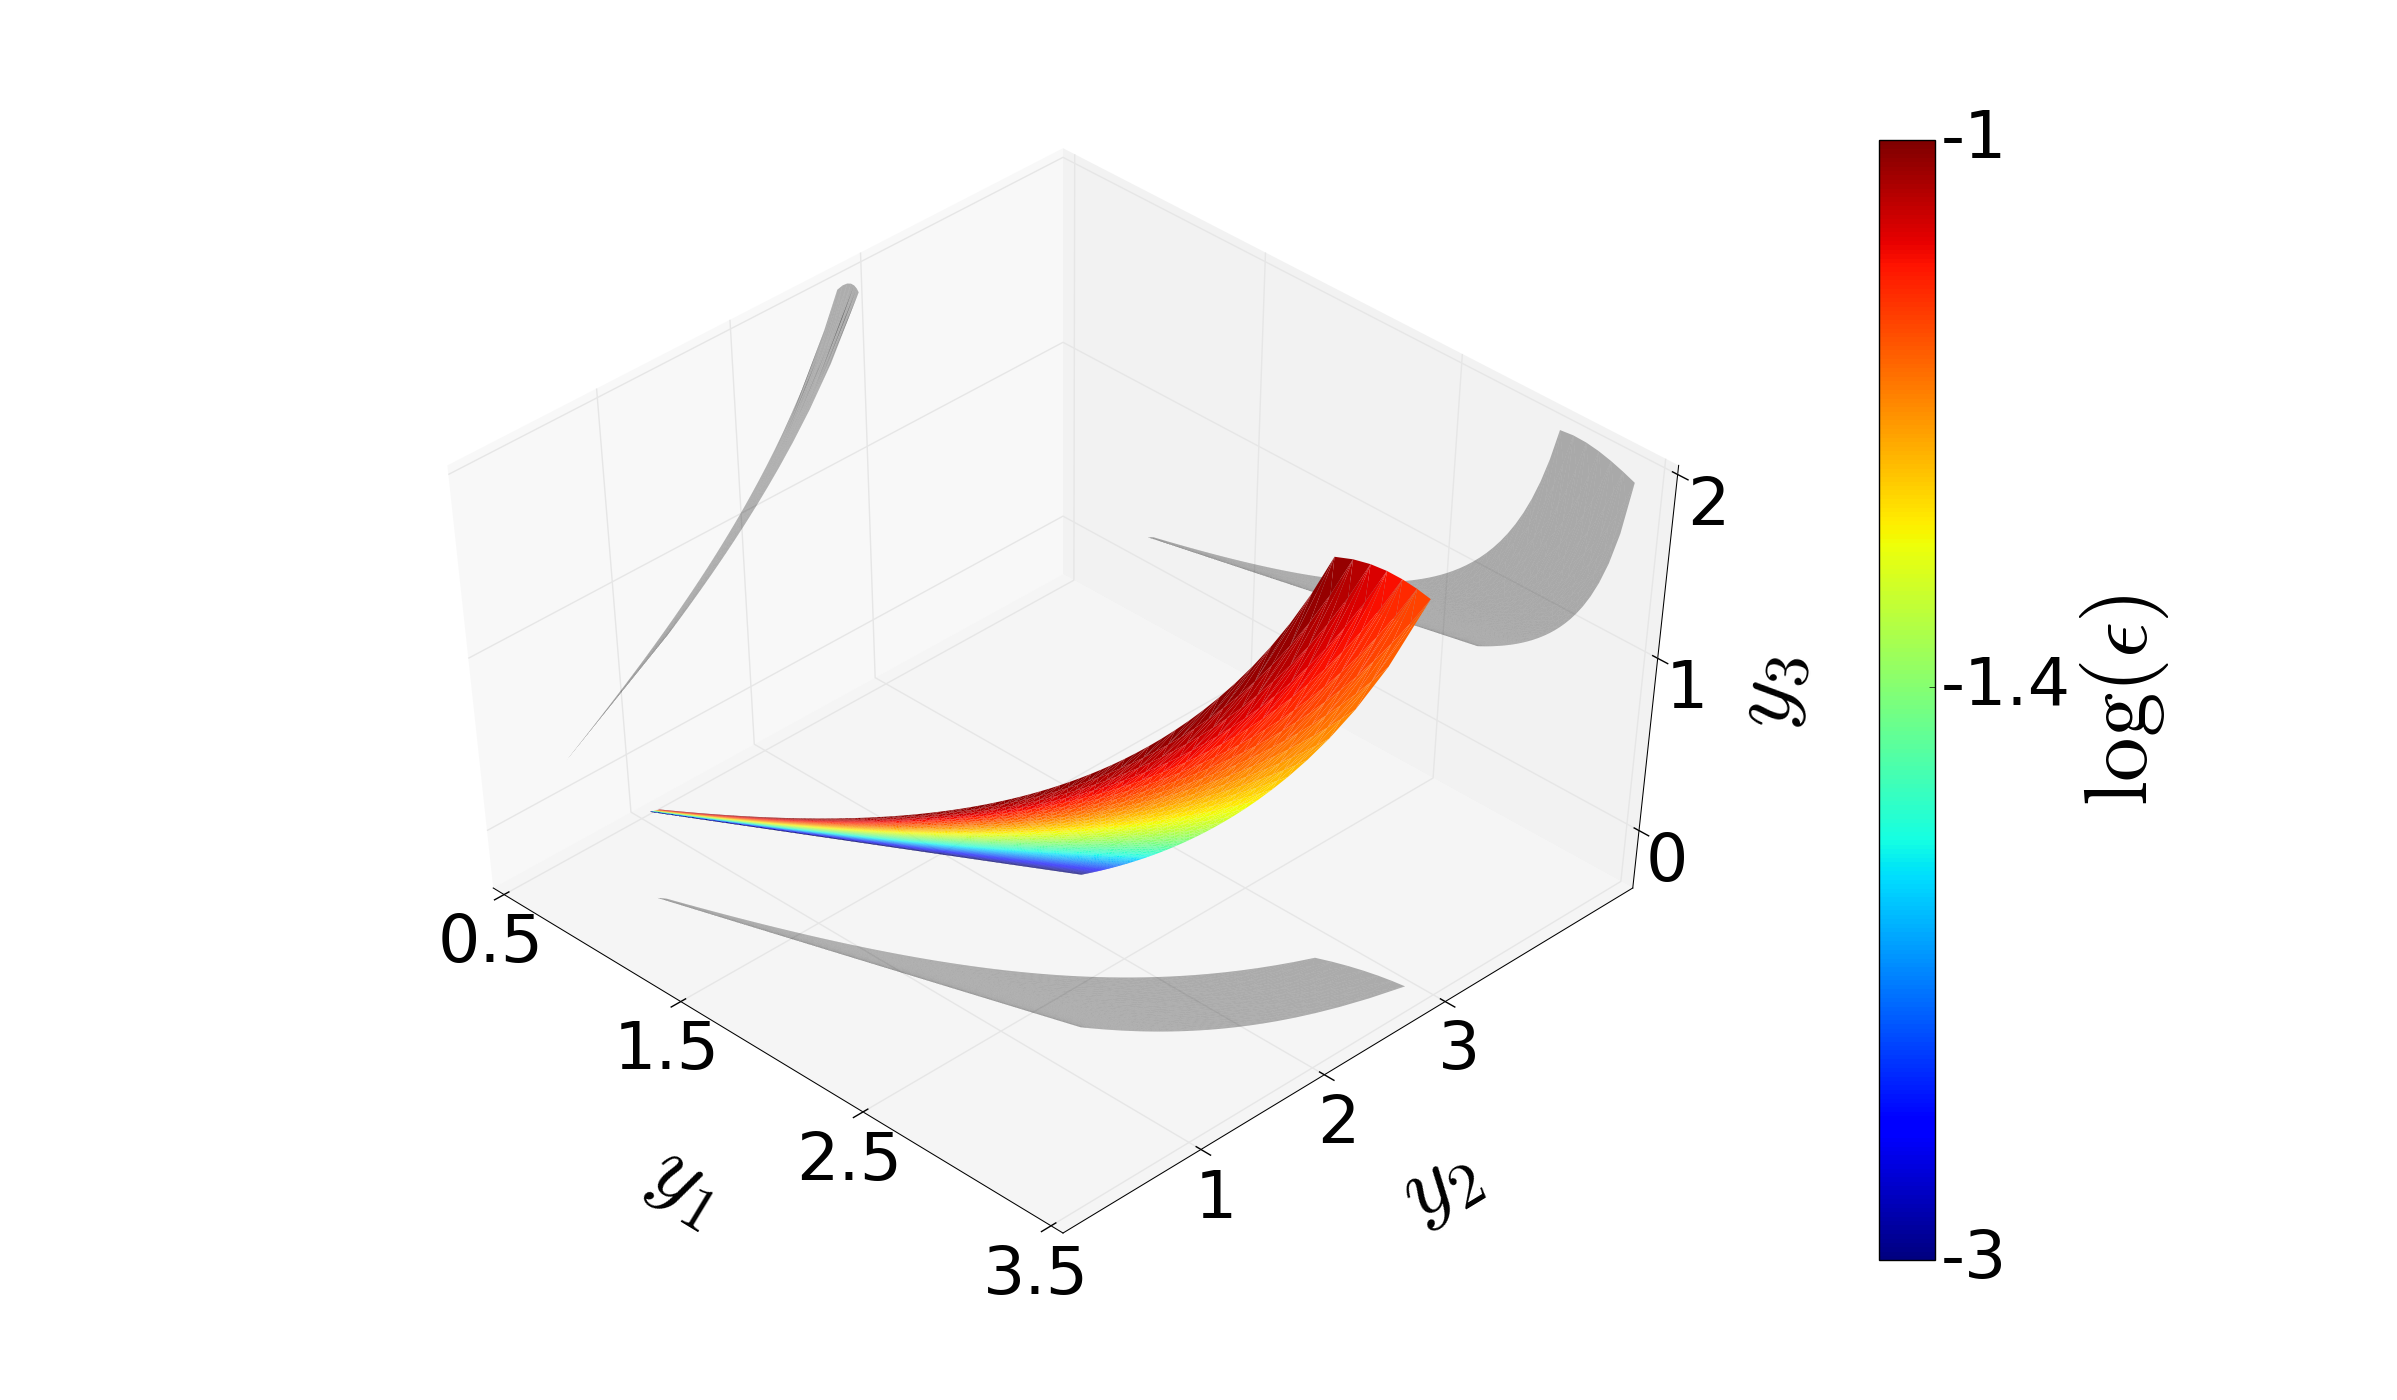
\includegraphics[width=0.5\textwidth]{y3-y2-y1-eps} &
                                                           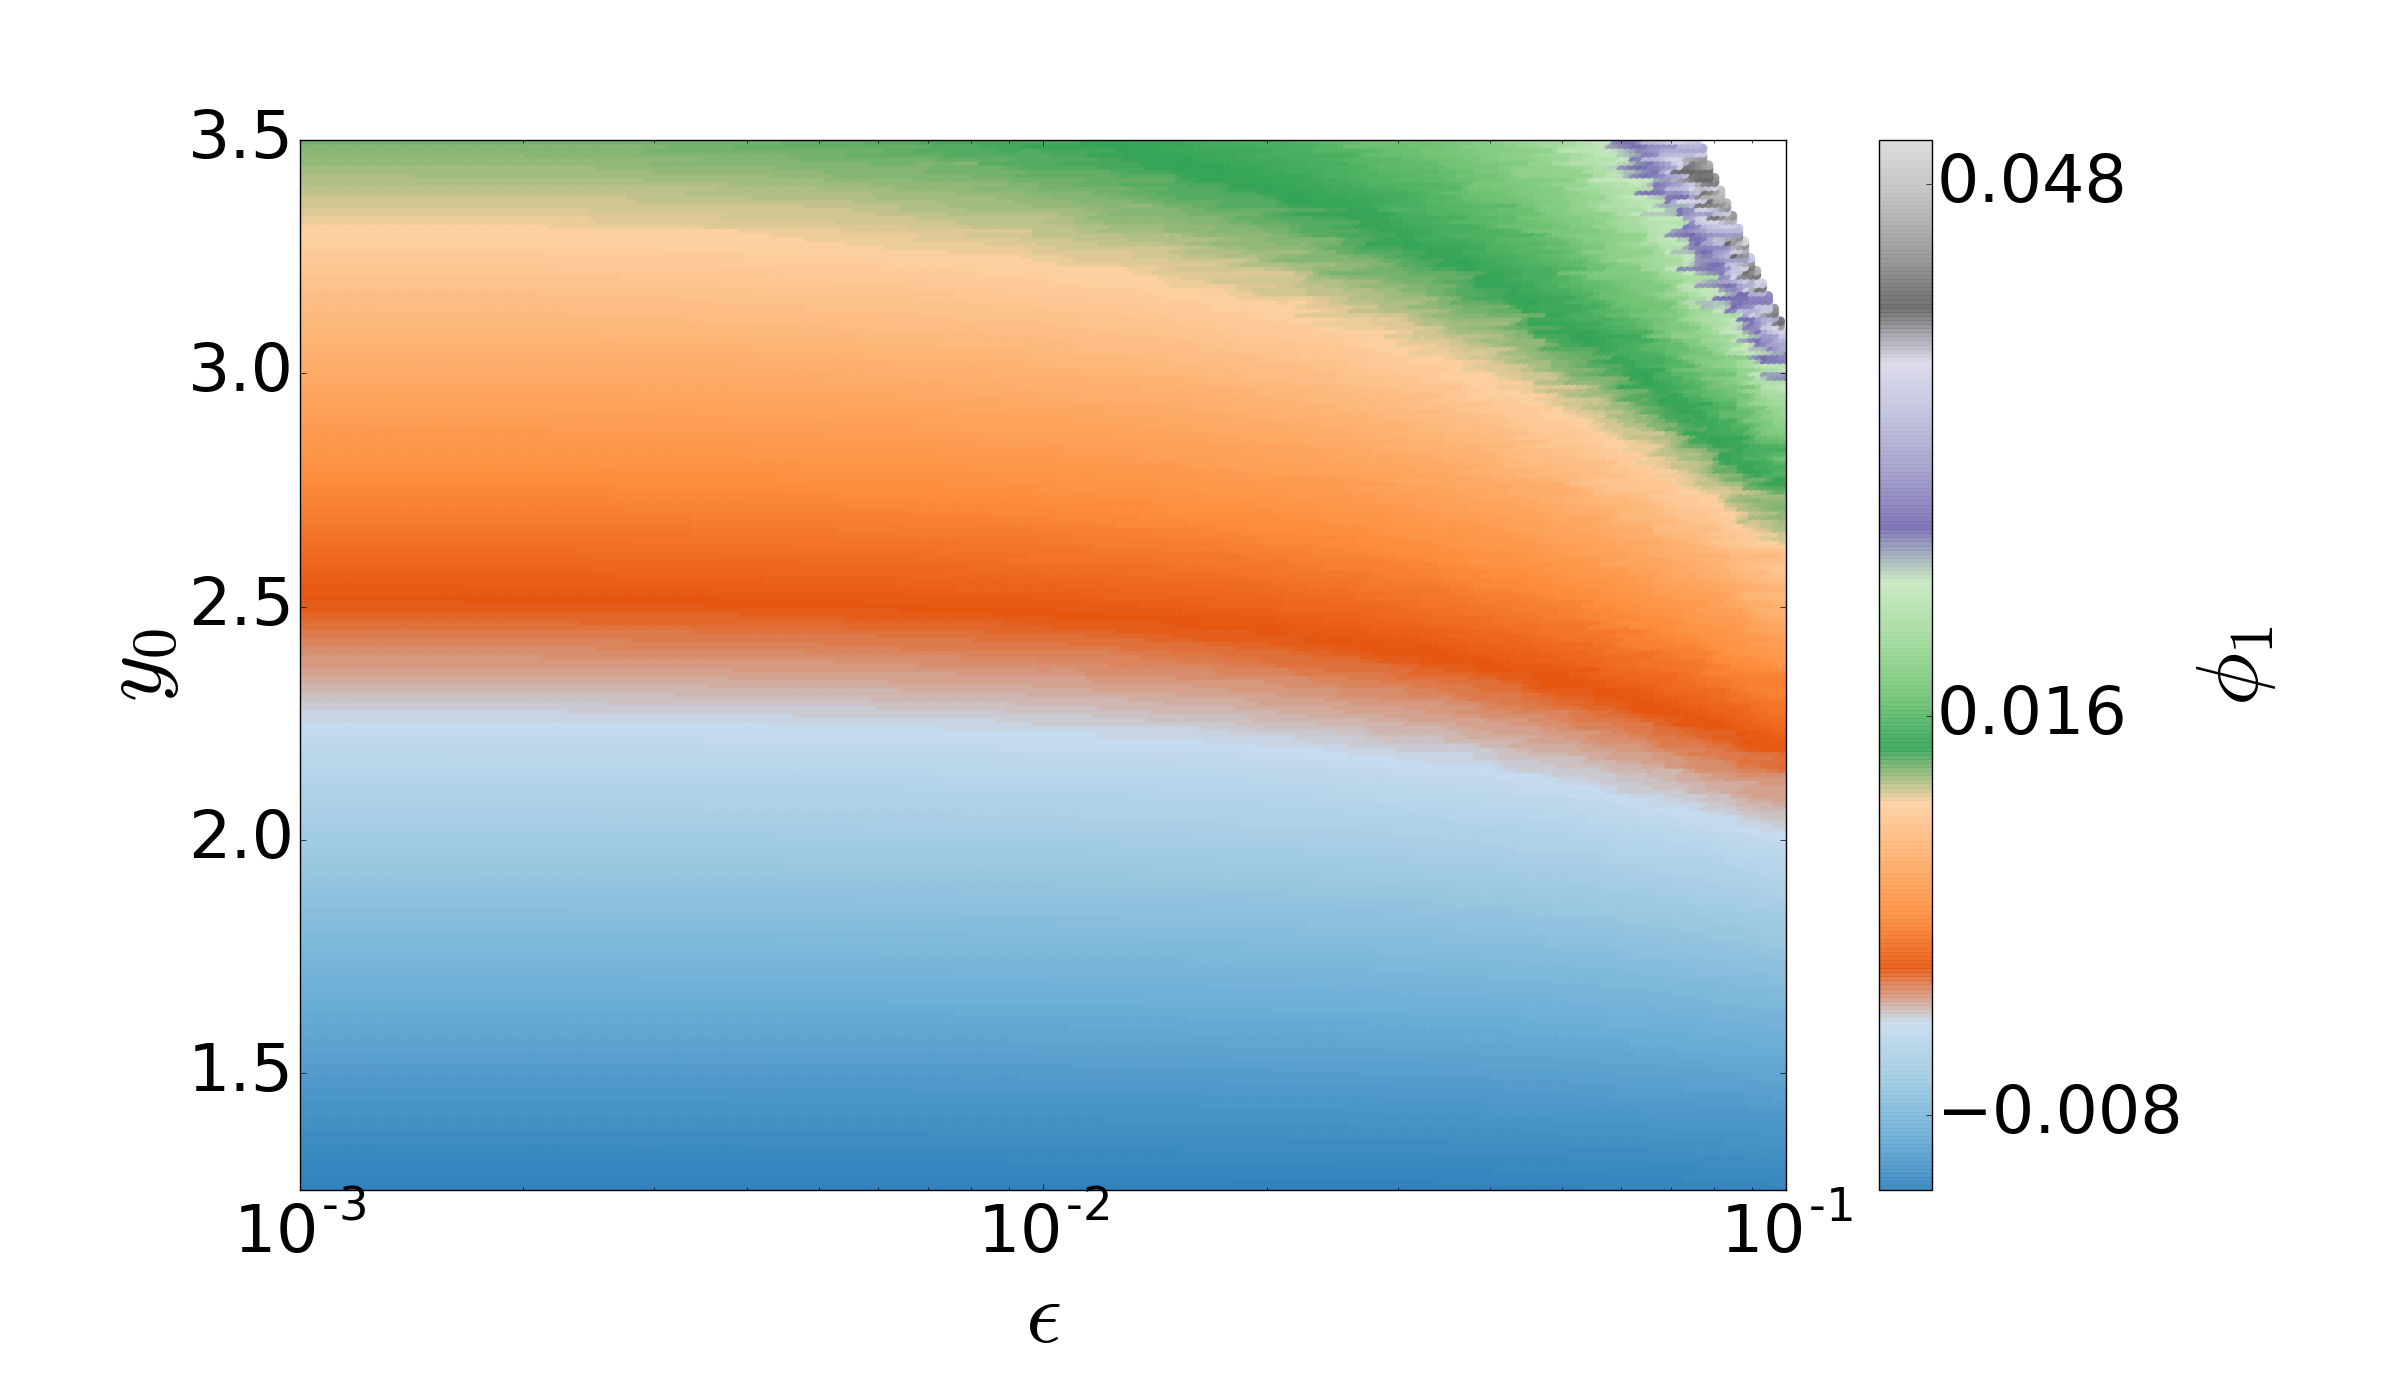
\includegraphics[width=0.5\textwidth]{y0-eps-phi1} \\
    (a) & (b)\\
  \end{tabular}
  \caption[Model manifold and parameter space of regularly perturbed system]{(a) Model manifold of regularly perturbed system with
    parameters $y_0$ and $\epsilon$, colored by $\epsilon$. As
    $\epsilon$ decreases, the model response is increasingly
    determined solely by $y_0$ as the system converges to $y' = -y$;
    (b) Parameter space colored by $\phi_1$ for the regularly
    perturbed system. As $\epsilon$ decreases, only the value of $y_0$
    is significant. This is captured by DMAPS as $\phi_1$ varies only
    vertically, in the $y_0$ direction, at small
    $\epsilon$. \label{fig:regpert}}
\end{figure}


\section{Singular perturbation}

The system is now given by

\begin{align}
  \frac{dx}{dt}&=2-x-y\\
  \frac{dy}{dt}&= \frac{1}{\epsilon}(x-y)
\end{align}    

with $\theta = (y_0, \epsilon)$ and
$f(\theta) = \left(y(t_1), y(t_2), \dots, y(t_n) \right)$ as
before. At small values of $\eps$ the equations become singularly
perturbed, and we cannot simply set $\eps = 0$ to find our reduced
description as before. Instead we see that $y$ will rapidly approach
the slow manifold $y = x$, and then progress towards the steady state
$(x,y) = (1,1)$. The phase portrait for this system is shown in
Figure~\ref{fig:singpert}.

Crucially, on the slow manifold our system is approximately
one-dimensional, governed by $\frac{dx}{dt} = -2 - 2x$. If we choose
our sampling times $t_1, t_2, \dots, t_n$ based on the slow timescale
of the system, our dynamics will be one-dimensional, and in fact
neither $\eps$ nor $y_0$ will affect the model response. At small
$\eps$, $y$ quickly converges to the slow manifold (order $\eps$
time), and then slowly evolves toward the stationary state. At
$\eps \ll 1$, our model manifold converges to a single,
zero-dimensional point. Whereas in the regularly perturbed example we
transitioned from two to one significant parameters, singular
perturbation brings a transition from two to zero. If we have obtained
a sample of the $(\eps, y_0)$ parameter plane, we can again apply
DMAPS to re-parameterize the system. Figure~\ref{fig:singpert-dmaps}
shows the results of such an analysis. In
Figures~\ref{fig:singpert-dmaps} (a) and (d) we have colored the
parameter plane by $\phi_1$ and $\phi_2$, analogous to
Figure~\ref{fig:regpert} (b). Both eigenvectors are constant at small
$\eps$ reflecting the complete absence of significant parameters in
this regime. At larger $\eps$, $\phi_1$ and $\phi_2$ vary
independently as this corresponds to the two-dimensional region of the
manifold. Both $(\eps, y_0)$ and $(\phi_1, \phi_2)$ can be used to
parameterize the system, but whereas there are distinct regions in
which $\eps$ and $y_0$ become irrelevant, $\phi_1$ and $\phi_2$ are
consistently significant. DMAPS provides an automated and improved
parameterization of the system.

To clarify the relationship between parameter space, the model
manifold and the DMAPS embedding, we plot these three views of the
singularly perturbed system in Figure~\ref{fig:singpert-patches}. We
also color four different patches and track their transformation from
one space to the next. The yellow rectangle at larger $\eps$ is mapped
to a slightly deformed rectangle in both the model manifold and DMAPS
embedding. The blue patch, which approaches the singularly perturbed
regime, becomes stretched at the tip. The red patch is compressed to
an apparently one-dimensional line, while the green patch, lying
solidly within the singularly perturbed region, is mapped to a single
point in both alternative spaces. This represents the fact that in the
limit of small $\eps$, neither $y_0$ nor $\eps$ influence the model
output: everything collapses to a zero-dimensional point.

\vspace{1cm}
\begin{figure}[!htp]
  \centering
  \includegraphics[width=0.4\textwidth]{sample_traj_sing}
  \caption[Phase portrait for singularly perturbed system]{The phase portrait of the singularly perturbed system for
    different initial conditions; solid lines: $\epsilon=0.02$, dotted
    lines are $\epsilon=0.12$. \label{fig:singpert}}
\end{figure}

\begin{figure}[!htp]
  \centering
  \begin{tabular}{ccc}
    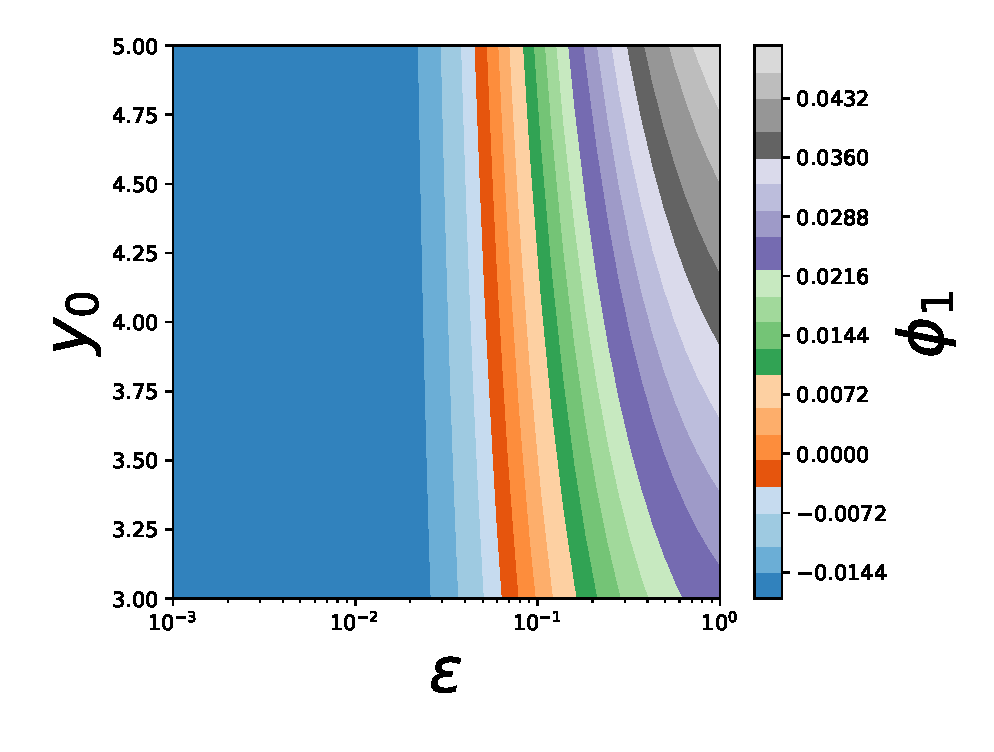
\includegraphics[width=0.33\textwidth]{y0_eps_phi1_sing} &
                                                               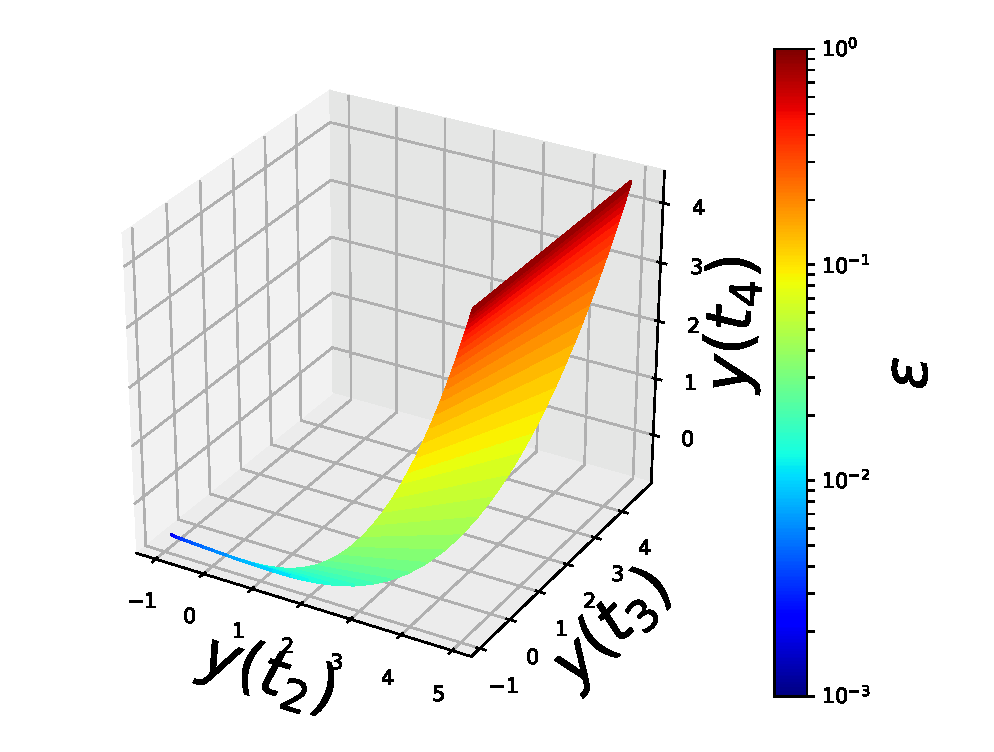
\includegraphics[width=0.33\textwidth]{mod_man_epsilon} &
                                                                                                                         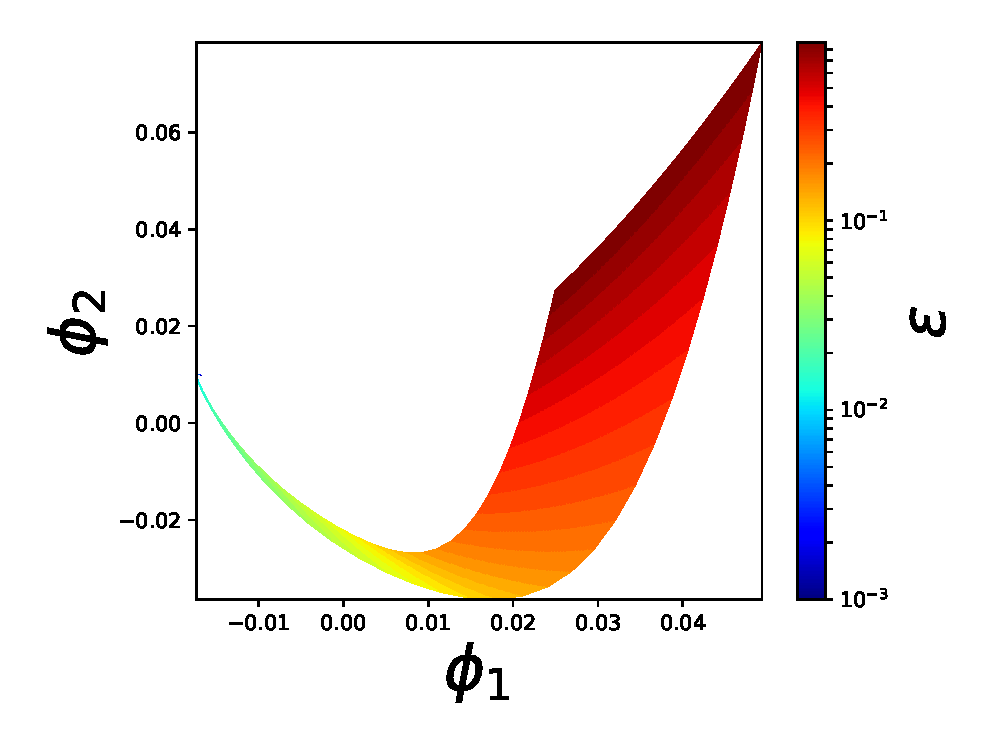
\includegraphics[width=0.33\textwidth]{phi2_phi1_eps_sing} \\
    (a) & (b) & (c)\\
    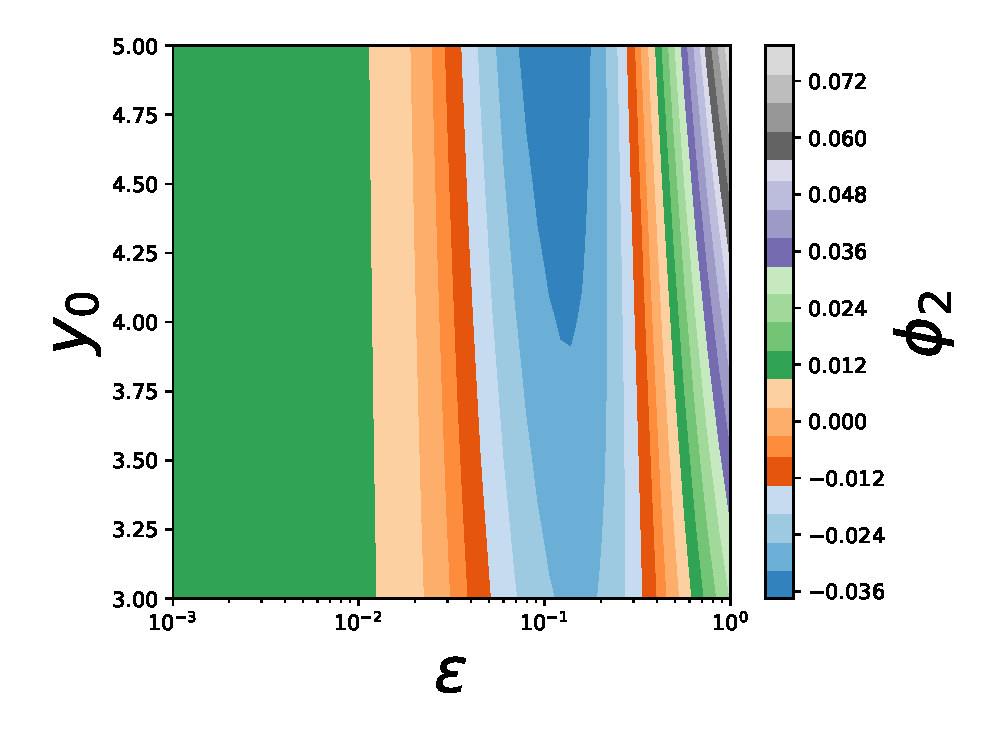
\includegraphics[width=0.33\textwidth]{y0_eps_phi2_sing} &
                                                               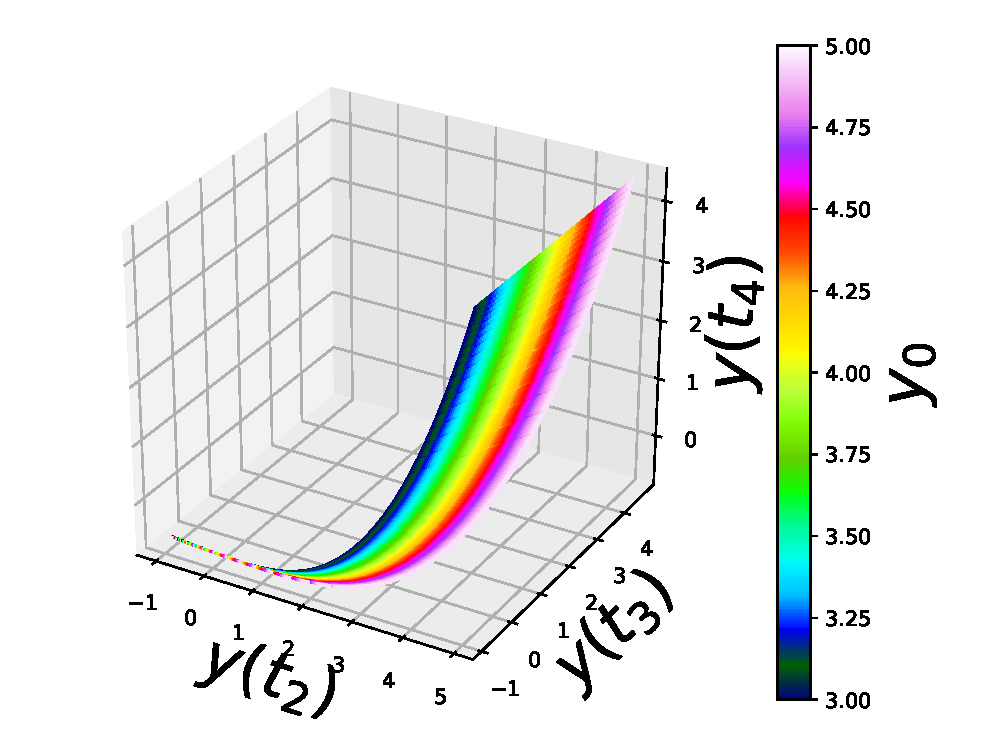
\includegraphics[width=0.33\textwidth]{mod_man_y0} &
                                                                                                                    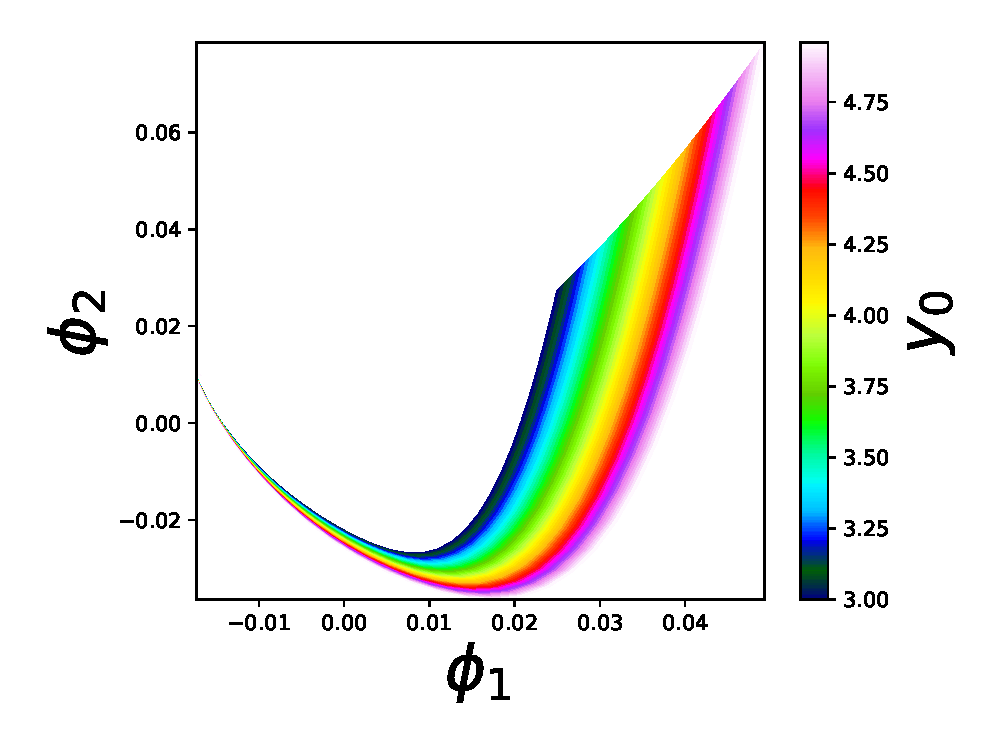
\includegraphics[width=0.33\textwidth]{phi2_phi1_y0_sing}  \\
    (d) & (e) & (f)\\
  \end{tabular}
  \caption[DMAPS results for singularly perturbed system]{(a) and (d) Parameter space colored by $\phi_1$ and
    $\phi_2$; (b) and (e) Model manifold colored by $\epsilon$ and
    $y_0$; (c) and (f) Diffusion map space colored by $\epsilon$ and
    $y_0$ \label{fig:singpert-dmaps}}
\end{figure}


\begin{figure}[!htp]
  \centering
  \begin{tabular}{c}
    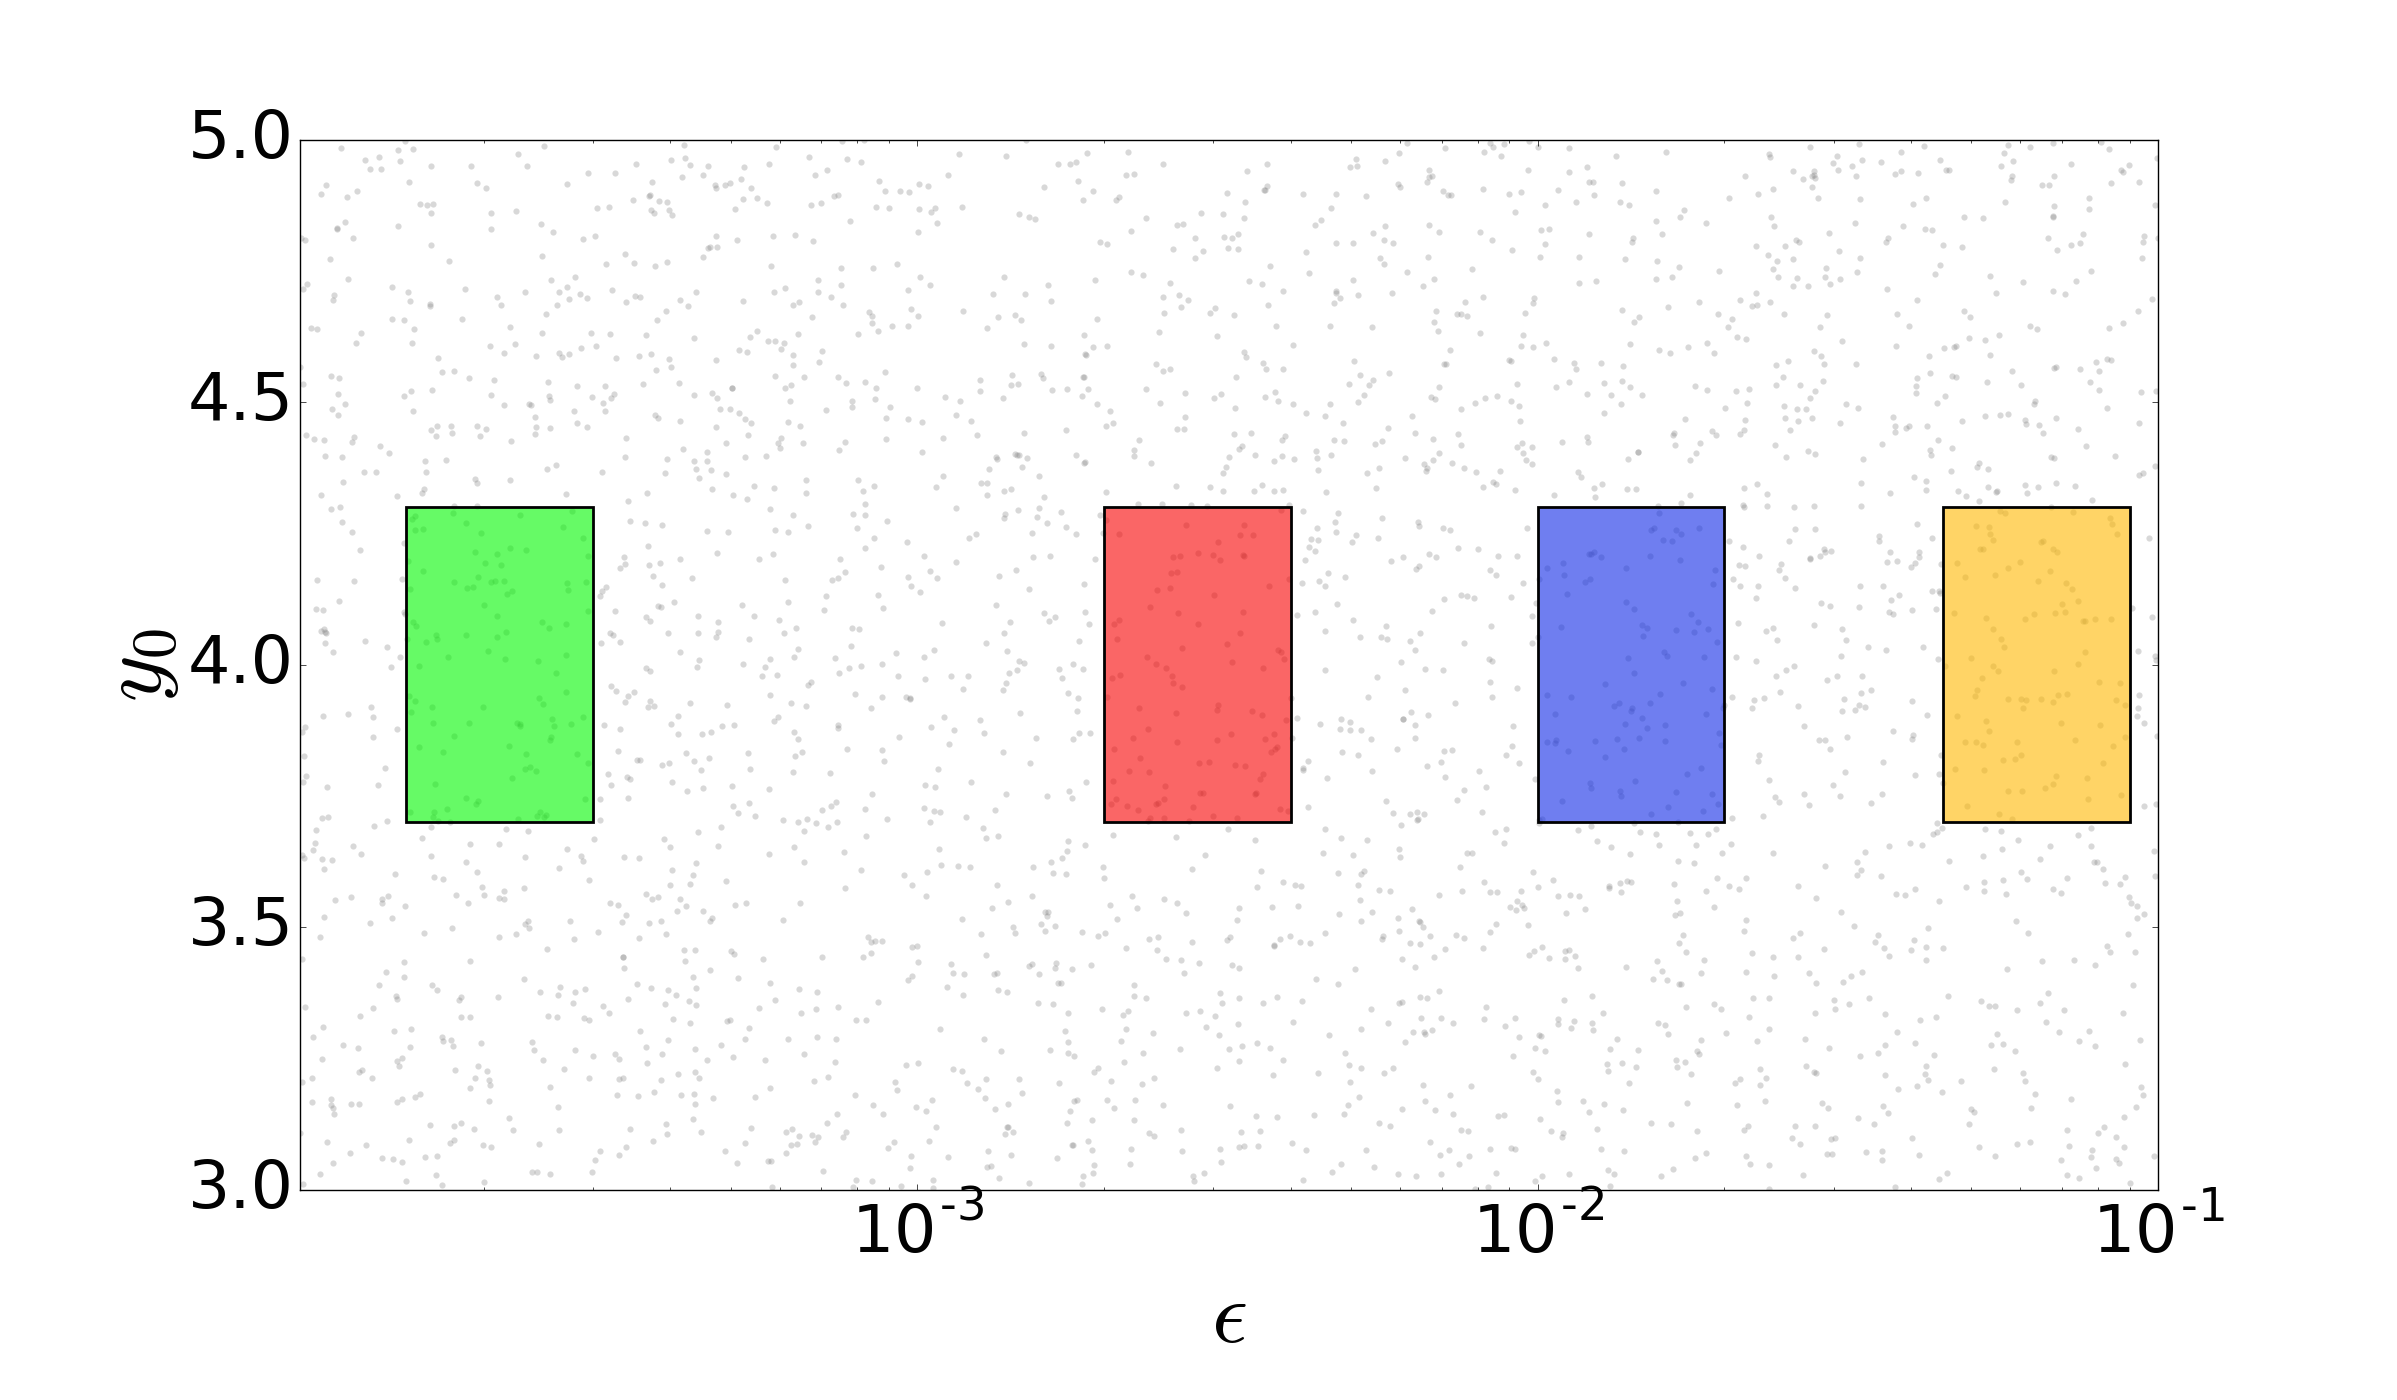
\includegraphics[height=0.2\textheight]{y0-eps-patches} \\
    (a)\\
    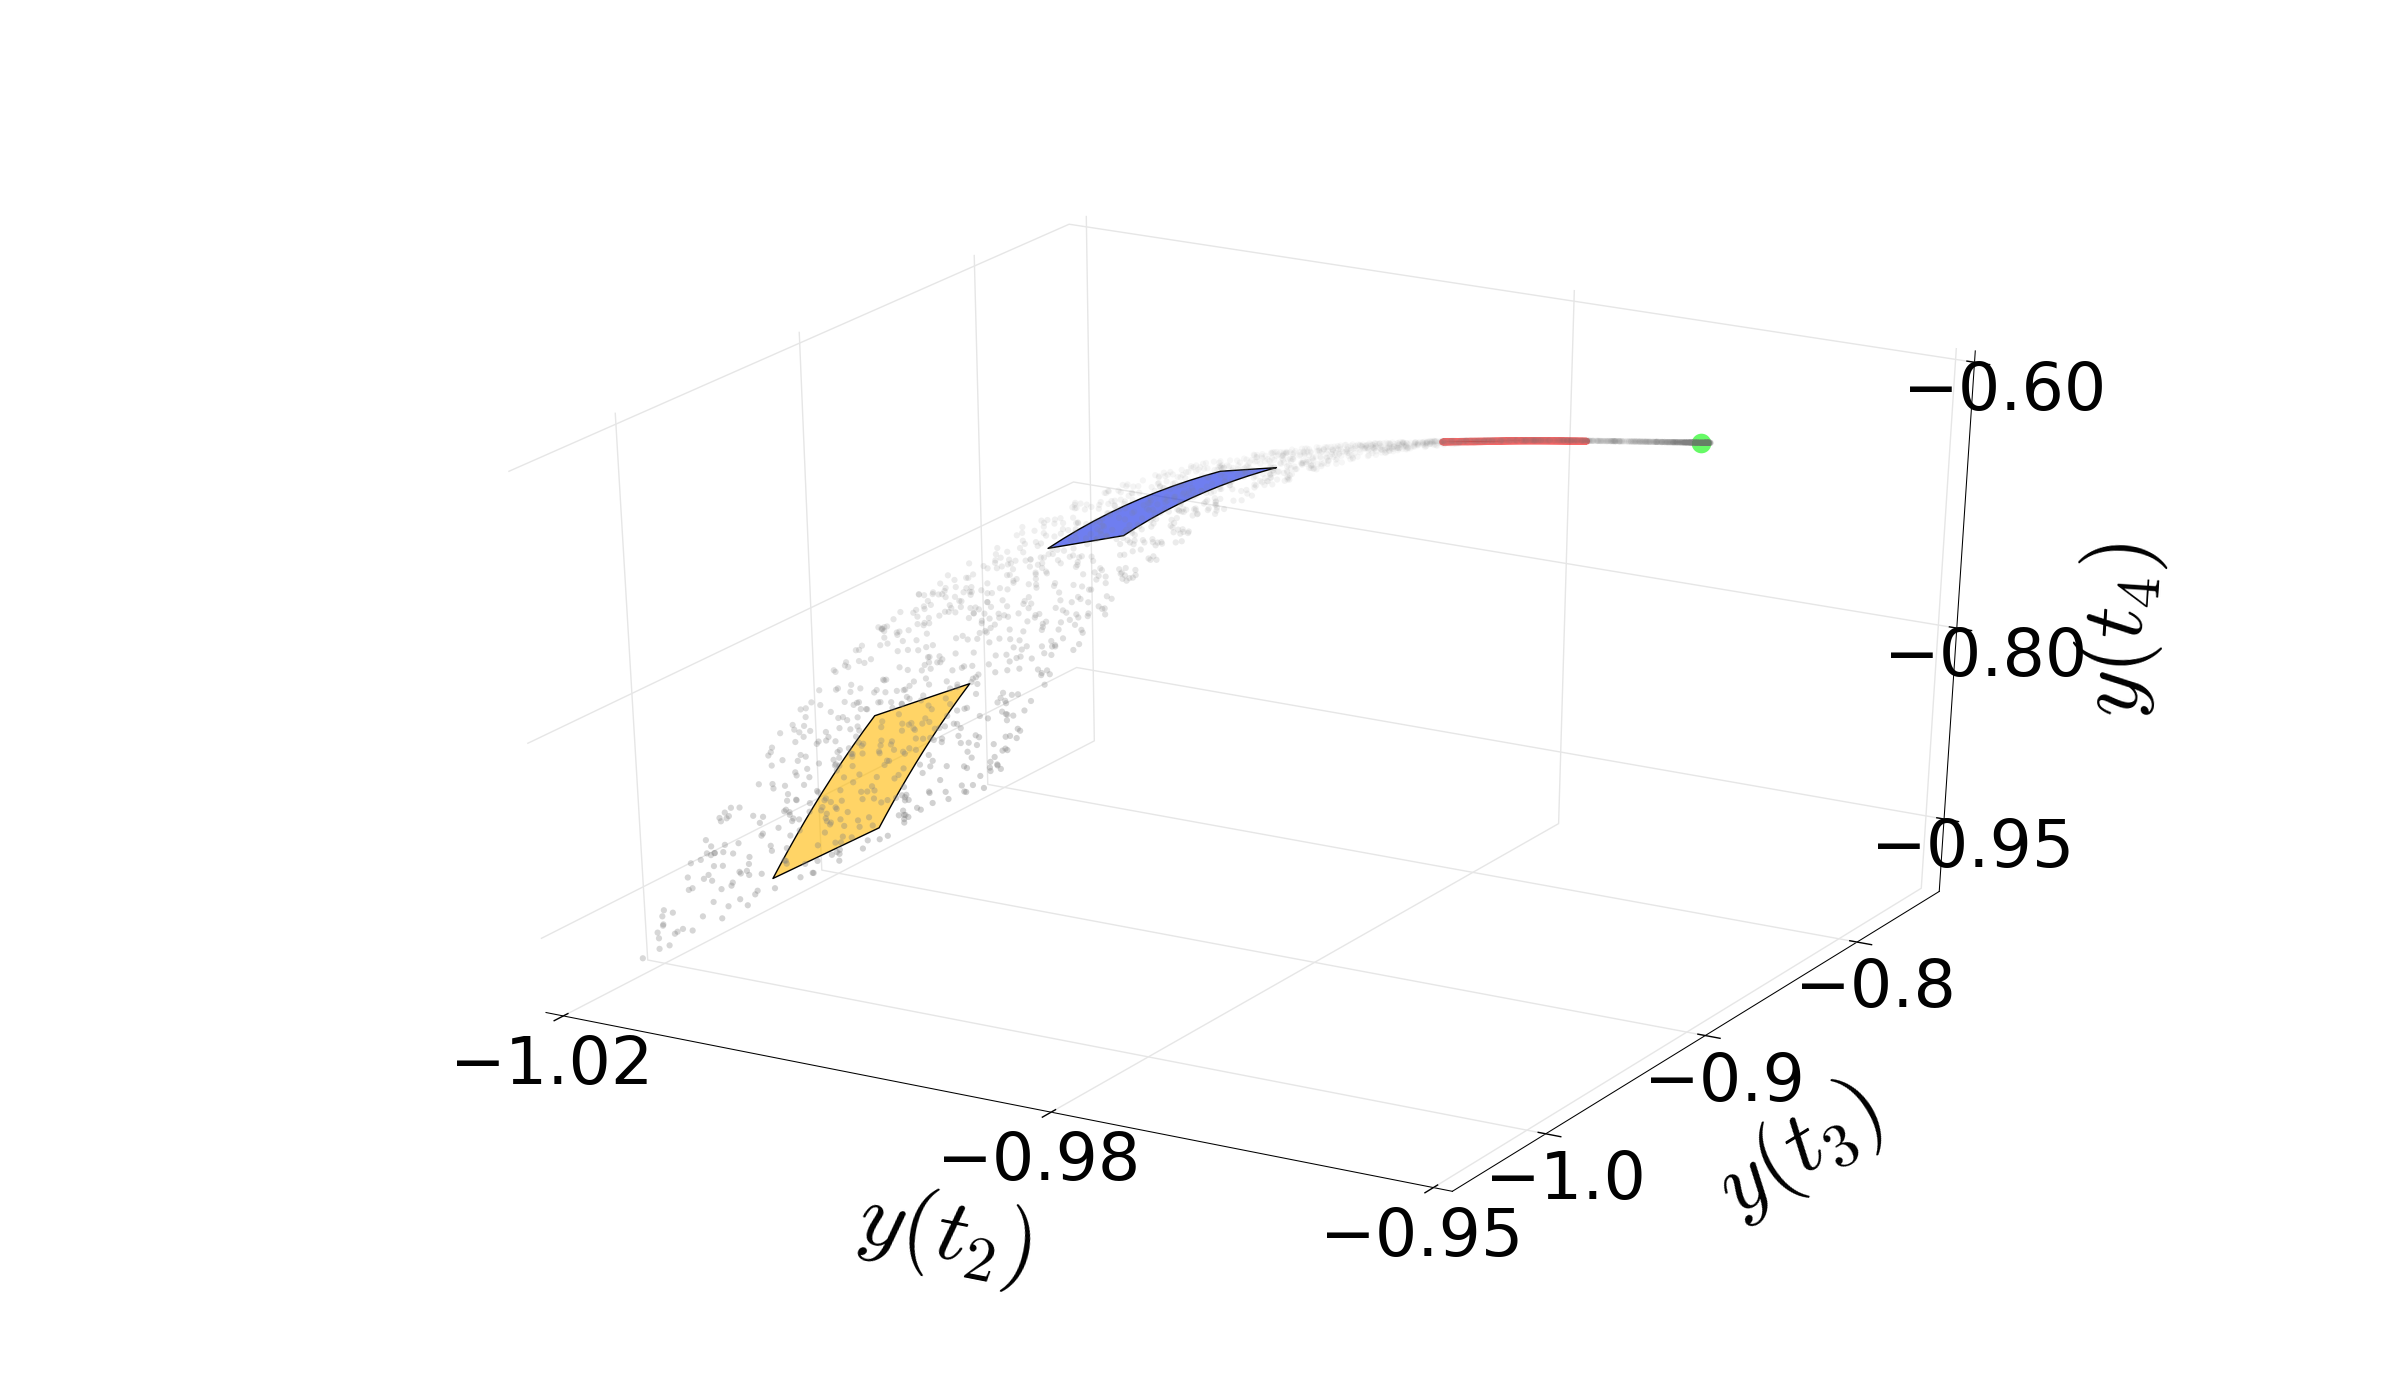
\includegraphics[height=0.2\textheight]{y4-y3-y2-patches}\\
    (b)\\
    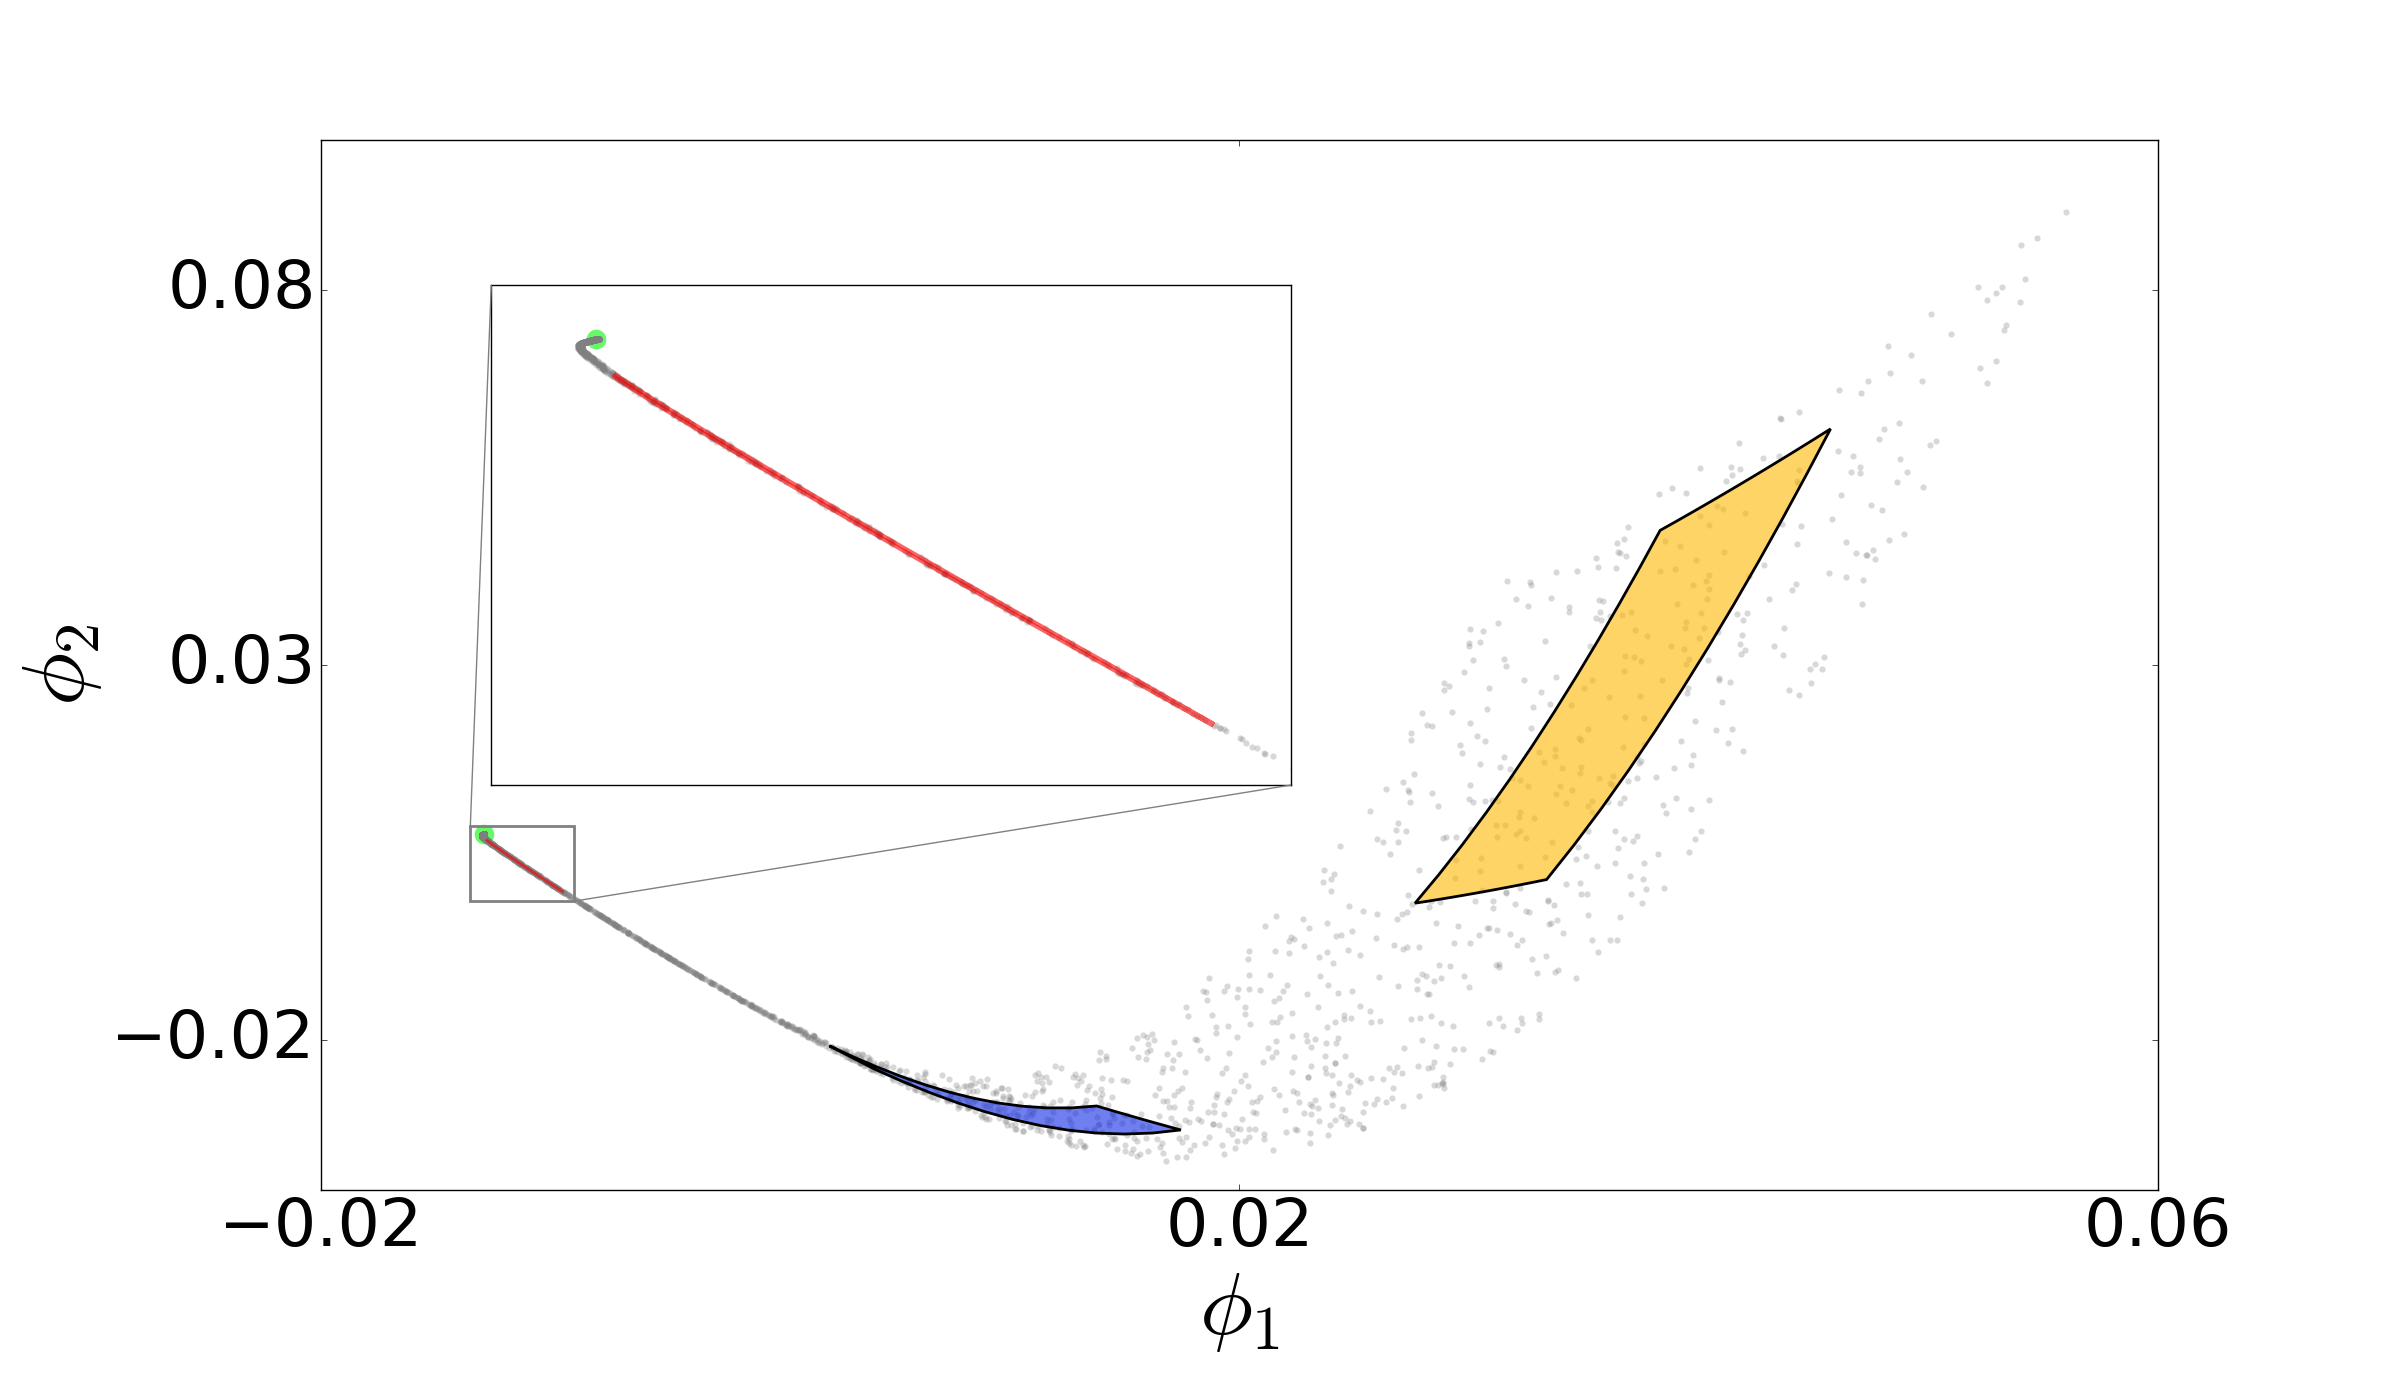
\includegraphics[height=0.2\textheight]{phi2-phi1-patches}\\
    (c)\\
  \end{tabular}
  \caption[Different views of singularly perturbed system]{(a) Patches in parameter space for the singularly perturbed
    system; (b) Corresponding patches in model response space; (c)
    Corresponding patches in DMAPS embedding
    space \label{fig:singpert-patches}}
\end{figure}


\section{Application to Michaelis-Menten kinetics}

Finally, we apply our toolbox to a familiar chemical kinetic
prototype, namely the Michaelis-Menten system modeling enzymatic
action \cite{johnson_original_2011}.  In that mechanism, a substrate
$S$ is turned into product $P$ by the action of an enzyme $E$ through
the creation of an intermediate complex $C$,

\begin{align}
  E + S \xrightleftharpoons[k_{-1}]{k_1} C \xrightarrow[]{k_2} E + P
  \label{mech:mm}
\end{align}

The mechanism differs from Mechanism~\ref{mech:abc} in that the
addition of a recycled but limited enzyme supply introduces
nonlinearities into the governing system of differential equations,


\begin{align}
  \begin{split}
    S' &= -k_1 E S + k_{-1} C , \\
    C' &= k_1 E S - (k_{-1} + k_2) C , \\
    E' &= -k_1 E S + (k_{-1} + k_2) C , \\
    P' &= k_2 C
  \end{split}
\end{align}


The conservation laws $S + P + C = S_T$ and $E + C = E_T$ reduce the
number of variables by two, and we arrive at the final model

\begin{align}
  \begin{split}
    S' &= -k_1 (E_T-C) S + k_{-1} C , \\
    C' &= k_1 (E_T-C) S - (k_{-1} + k_2) C
    \label{eq:MM}
  \end{split}
\end{align}

Following the classical setting
\cite{johnson_original_2011,johnson_original_2011,segel_quasi-steady-state_1989},
we set the initial concentrations of complex and product to zero,
$C_0=P_0=0$, so that $S_0 = S_T$ and $E_0 = E_T$.  Further adapting
ideas from \cite{segel_quasi-steady-state_1989}, we recoordinatize the
parameter space through the transformations

\begin{align}
  \begin{split}
    K_M = \dst\frac{k_{-1} + k_2}{k_1} , &\quad
    V_M = k_2 E_T , \\
    \sigma = \dst\frac{S_T}{K_M} , \quad \kappa =
    \dst\frac{k_{-1}}{k_2} , &\quad \epsilon = \dst\frac{E_T}{S_T +
      K_M}
    \label{eq:param-defs}
  \end{split}
\end{align}

The observable here is the product concentration $P$ at ten equally
spaced times in the interval $[t_s/2,2t_s]$, where the timescale
$t_s = (S_T^* + K_M^*)/V_M^*$. Thus
$f:\mathbb{R}^5 \rightarrow \mathbb{R}^{10}$ maps our five
parameter values to ten points along $P$'s trajectory. Setting
reference parameter values at
$(K_M^*,V_M^*,S_T^*,\epsilon^*,\kappa) = (1,1,1,10^{-3},10)$, we
investigate the system in a manner similar to that previously
presented.  First we sample parameter settings lying within a fixed
distance $\delta=0.05$ of
$f^* = f(K_M^*, V_M^*, S_T^*, \epsilon^*,
\kappa^*)$, and then we apply the modified DMAPS algorithm to that
dataset to uncover significant parameter combinations.  Before delving
into DMAPS, however, we first probe the system with a simpler, linear
PCA analysis.  By applying this technique to the Jacobian of the model
response

\begin{align}
  \mathrm{J} = \begin{bmatrix} \frac{\partial f_1}{\partial K_M} &
    \frac{\partial f_1}{\partial V_M} & \frac{\partial f_1}{\partial
      S_T} & \frac{\partial f_1}{\partial \epsilon} & \frac{\partial
      f_1}{\partial \kappa} \\ \vdots & & & & \vdots \\ \frac{\partial
      f_N}{\partial K_M} & & \hdots & & \frac{\partial f_N}{\partial
      \kappa} \end{bmatrix}
\end{align}

and examining the coefficients of the principal components
$\mathrm{V}$ where $\mathrm{J} = \mathrm{U \Sigma V^T}$, we will
uncover, in a local, linear sense, a basis for parameter space which
better captures the directions which do and do not affect model
output. This can be observed from the fact that
$\| f(\theta + \Delta \theta) - f(\theta) \| \approx \| \mathrm{J}
\Delta \theta \| = \| \mathrm{U \Sigma V^T} \Delta \theta
\|$. When $\Delta \theta$ aligns with a principal component whose
corresponding singular value is large, it will point in a direction of
significant model response variation. Conversely, a
$\Delta \theta$ which aligns with a principal component whose
singular value is small will point in a sloppy direction along which
model response changes minimally. Examining the SVD of the Jacobian
evaluated at $\theta^*$ we find for the principal components (with
entries less than $10^{-1}$ rounded to zero and singular values
rounded to the nearest order of magnitude for clarity)

\[
  V = \begin{blockarray}{cccccc} & v_1 & v_2 & v_3 & v_4 & v_5
    \\ \begin{block}{c[ccccc]} K_M & 0.3 & \minus 0.4 & \minus 0.9 & 0
      & 0 \\ V_M & \minus 0.4 & 0.8 & \minus 0.5 & 0 & 0 \\ S_T &
      \minus 0.9 & \minus 0.5 & 0 & 0 & 0 \\ \epsilon & 0 & 0 & 0 &
      0.9 & \minus 0.5 \\ \kappa & 0 & 0 & 0 & \minus 0.5 & \minus 0.9
      \\ \end{block} & & & & & \\ \begin{block}{c[ccccc]} \sigma &
      10^0 & 10^0 & 10^{\minus 2} & 10^{\minus 5} & 10^{\minus 6}
      \\ \end{block} \end{blockarray}
\]

where the final row labeled $\sigma$ contains the corresponding
singular values. This simple analysis immediately suggests the
existence of two sloppy parameters in this regime, $\kappa$ and
$\epsilon$, as the principal components that span these axes
correspond to significantly smaller singular values compared to the
other vectors. In addition, it appears that the parameter space
direction $K_M = V_M$ may be sloppy as this approximately corresponds
to the third smallest principal component, singular value pair. With
this simple analysis in hand, we turn to computational verification of
the results using both direct numerical experiments and the DMAPS
scheme outlined above, along with supporting analytical arguments.

First we show that the direction $K_M = V_M$ is indeed sloppy so that
one cannot precisely determine both $K_M$ and $V_M$, but only their
ratio. To do so we turn to the Lineweaver-Burk plot, a graphical
procedure allowing one to determine $K_M$ and $V_M$ from experimental
data of the reaction rate and substrate concentration evolution over
time \cite{lineweaver_determination_1934}. By generating many noisy realizations of the product
concentration profiles as one might collect experimentally in the lab
and then fitting each with the Lineweaver-Burk method, we can observe
the range of predicted $K_M$, $V_M$ pairs. These results are plotted
in Fig.~\ref{fig:lb}. In a typical setting we would expect a spread of
predicted values centered around the true, zero-noise parameters
taking the shape of some ellipsoid. However, as we have seen in
previous examples, in the presence of sloppiness this ellipsoid would
be stretched out along the sloppy parameter direction. This is
precisely what we find in Fig.~\ref{fig:lb}: so long as the ratio
$K_M/V_M = K_M^*/V_M^* = 1$, a wide range of values provide best-fit
parameters in the presence of slight noise. Therefore, when fitting
parameters in this regime, we must accept that we may not be able to
determine precise values of both $K_M$ and $V_M$.


\begin{figure}
  \centering
  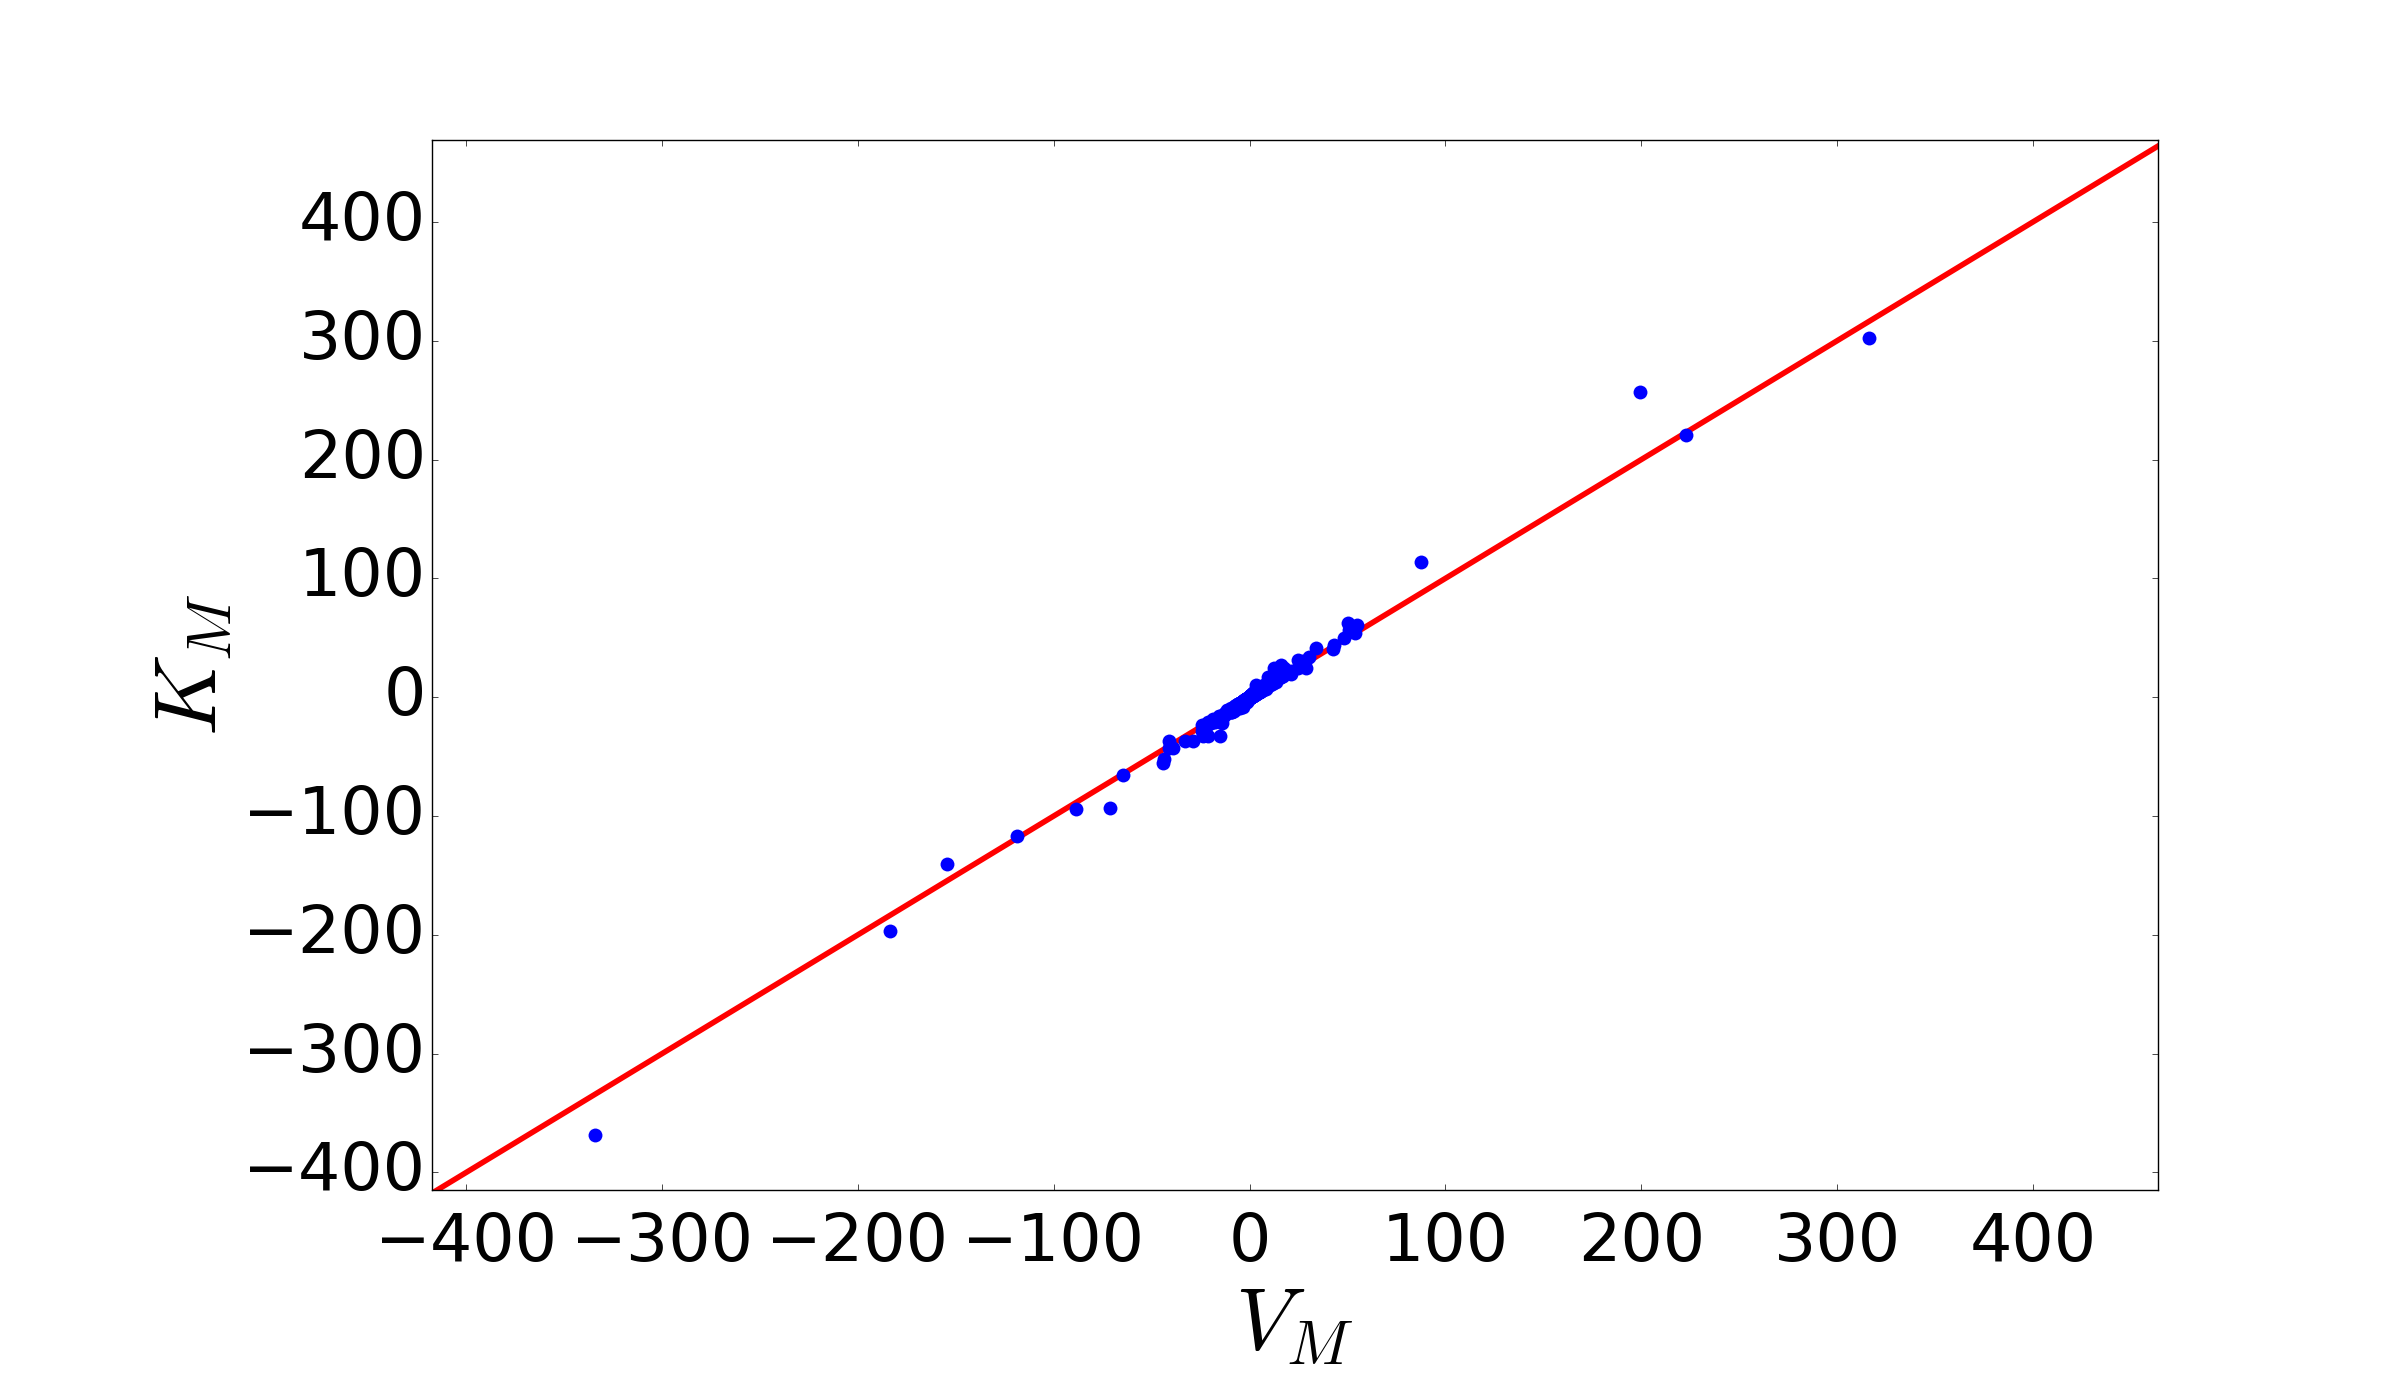
\includegraphics[width=1.0\linewidth]{k-v-lb}
  \caption[Lineweaver-Burk fitting results]{Best fit $K_M$ and $V_M$ values for many noisy
    concentration trajectories (blue dots). Sloppiness is evident in
    the spread of the data along the line $K_M/V_M = 1$ (plotted in
    red for reference). \label{fig:lb} }
\end{figure}

Next, we examine the system using DMAPS. We use the five-dimensional
dataset obtained by sampling parameter space around $\theta^*$ and
keeping those points for which
$\|f(\theta) - f(\theta^*) || < 5 \cdot 10^{-2}$, and apply DMAPS
with an $\epsilon$ value of $10^{-1}$.

Having computed our DMAP eigenvectors, it remains to determine which
of them correspond to independent directions in parameter space, as
certain eigenvectors may parameterize the same directions (see
\cite{dsilva_parsimonious_2015} for details). Using the algorithm
developed in \cite{dsilva_parsimonious_2015}, we compute a residual
for each eigenvector which, roughly speaking, assesses how much new
information it contains. The results shown in Fig~\ref{fig:resids}
suggest that eigenvectors $\phi_1$ and $\phi_2$ parameterize
independent directions. Our previous analysis would then suggest that
$\phi_1$ and $\phi_2$ correspond to important parameter directions,
and would provide a good set of coordinates on our model manifold.

We can test this hypothesis by projecting the model manifold onto two
axes, here $f_1$ and $f_{10}$, and coloring the result by our
eigenvectors. If the colors vary smoothly over the points, we have
uncovered an eigenvector that parameterizes the manifold. These
colorings are provided in Fig.~\ref{fig:mm-dmaps}. Based on these
figures, we can conclude that indeed $\phi_1$ and $\phi_2$ provide
coordinates along the model manifold. The sloppiness in $K_M/V_M$ was
discussed in the previous paragraph, but it remains to show why we
would lose two more parameters. In fact, as $\epsilon \rightarrow 0$,
the set of differential equations given in \eqref{eq:MM} become
singularly perturbed. In this limit, the leading order dynamics are
not influenced by $\kappa$, as shown in
\cite{segel_quasi-steady-state_1989}. Thus, for small enough
$\epsilon$, we will lose our ability to determine both $\epsilon$ and
$\kappa$. This is precisely what is reflected in our DMAPS results.

\begin{figure}[!htp]
  \centering
  \begin{tabular}{cc}
    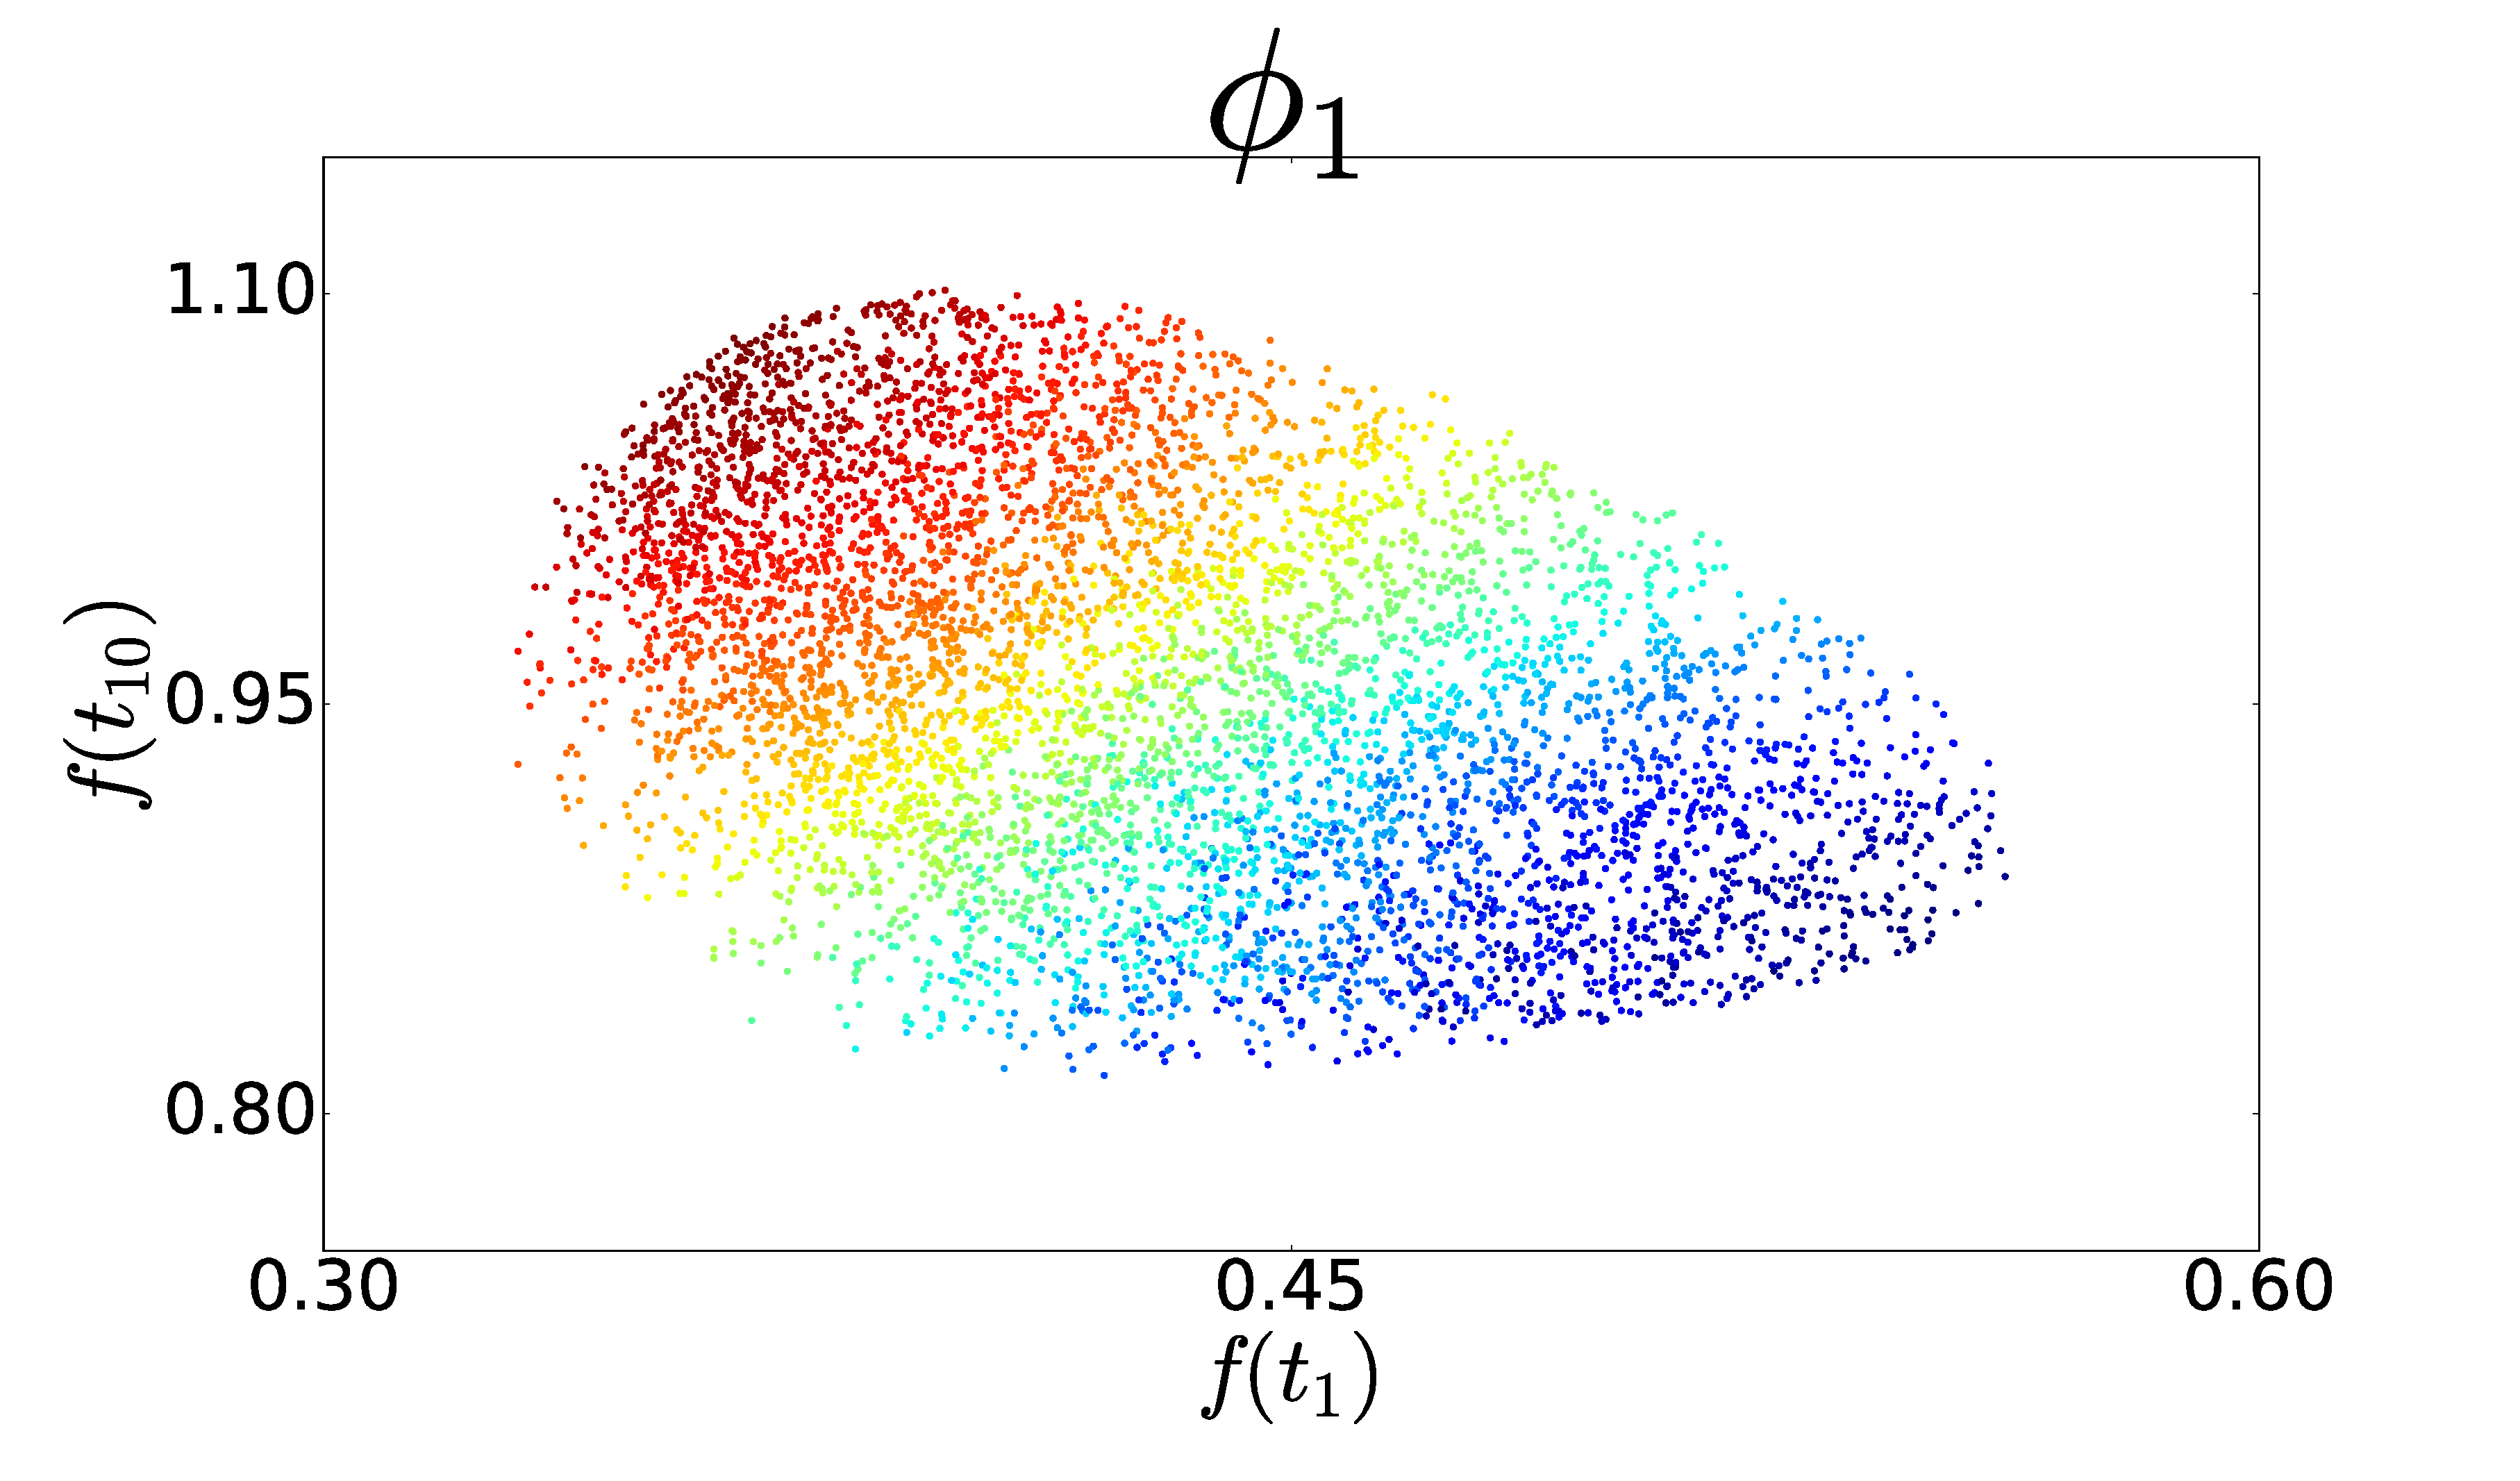
\includegraphics[width=0.5\textwidth]{f10-f1-phi1} &
    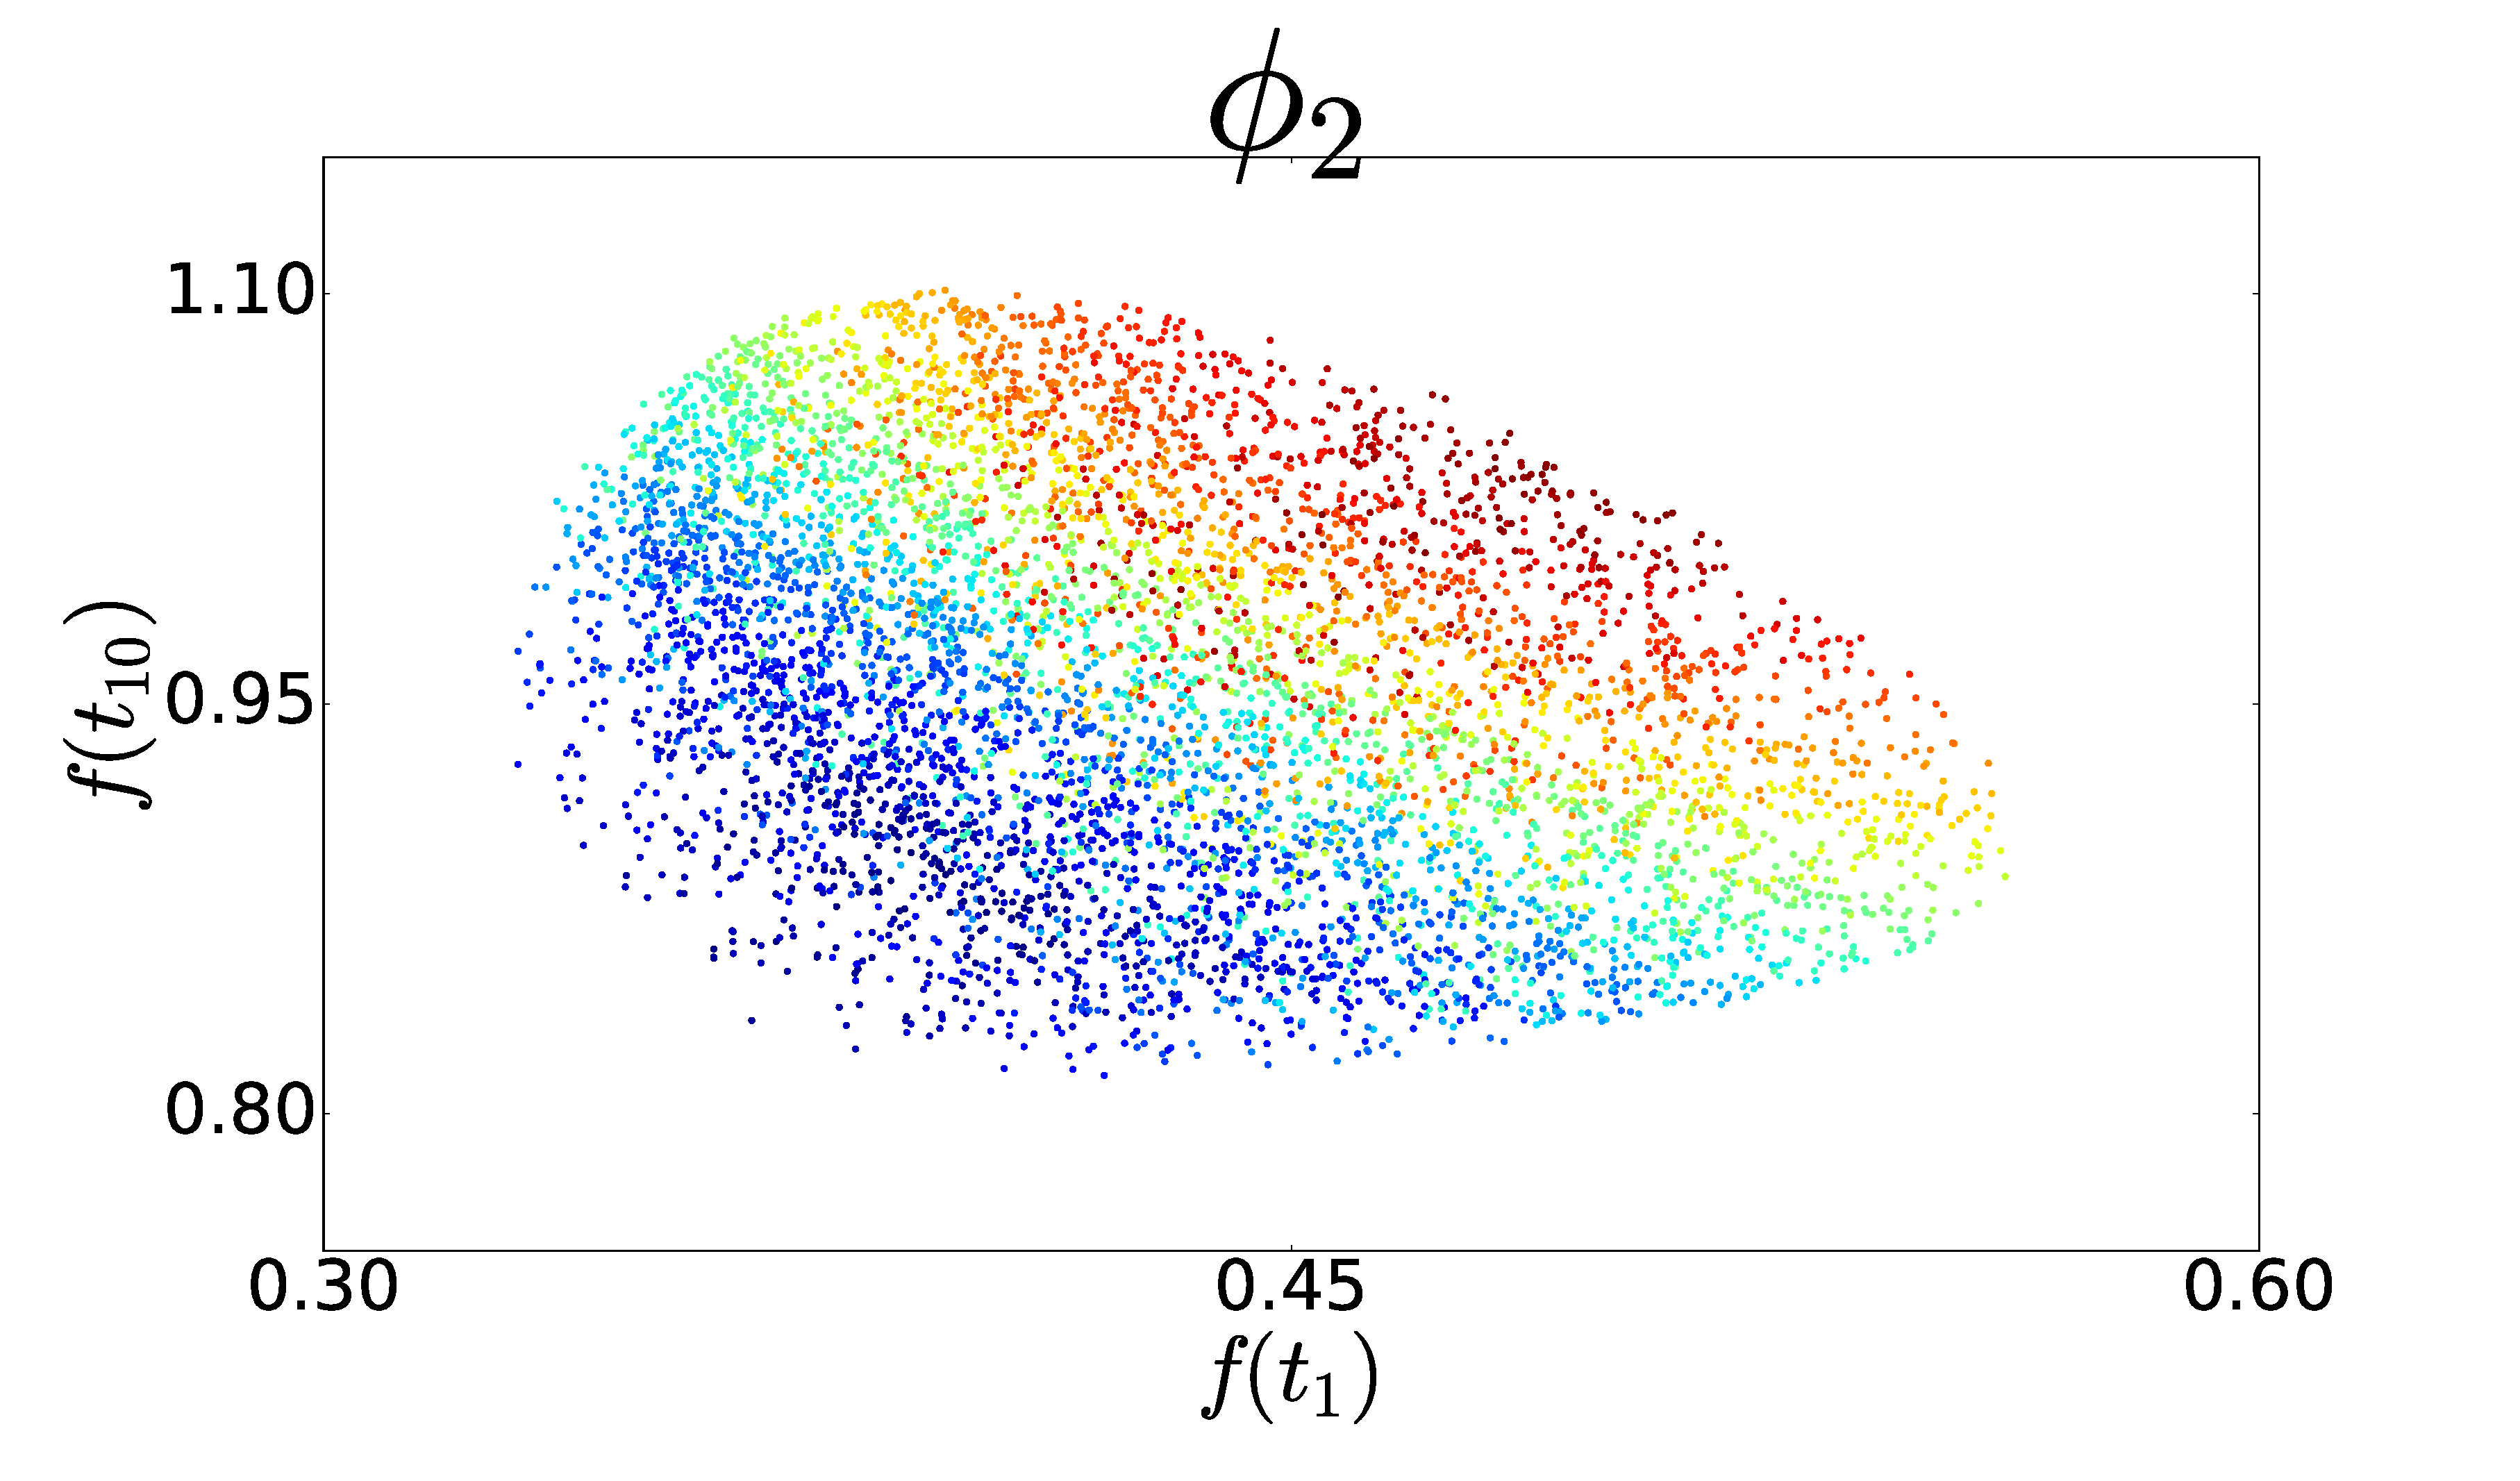
\includegraphics[width=0.5\textwidth]{f10-f1-phi2}\\
    (a) & (b) \\
  \end{tabular}
  \caption[DMAPS results for Michaelis-Menten system I]{Projection of the model manifold onto $f_1$ and $f_{10}$
    colored by different DMAP eigenvectors. As $\phi_1$ and $\phi_2$
    vary smoothly over the surface and parameterize independent
    directions, these eigenvectors offer a good pair of coordinates on
    the manifold \label{fig:mm-dmaps}}
\end{figure}


\begin{figure}[ht!]
  \centering
  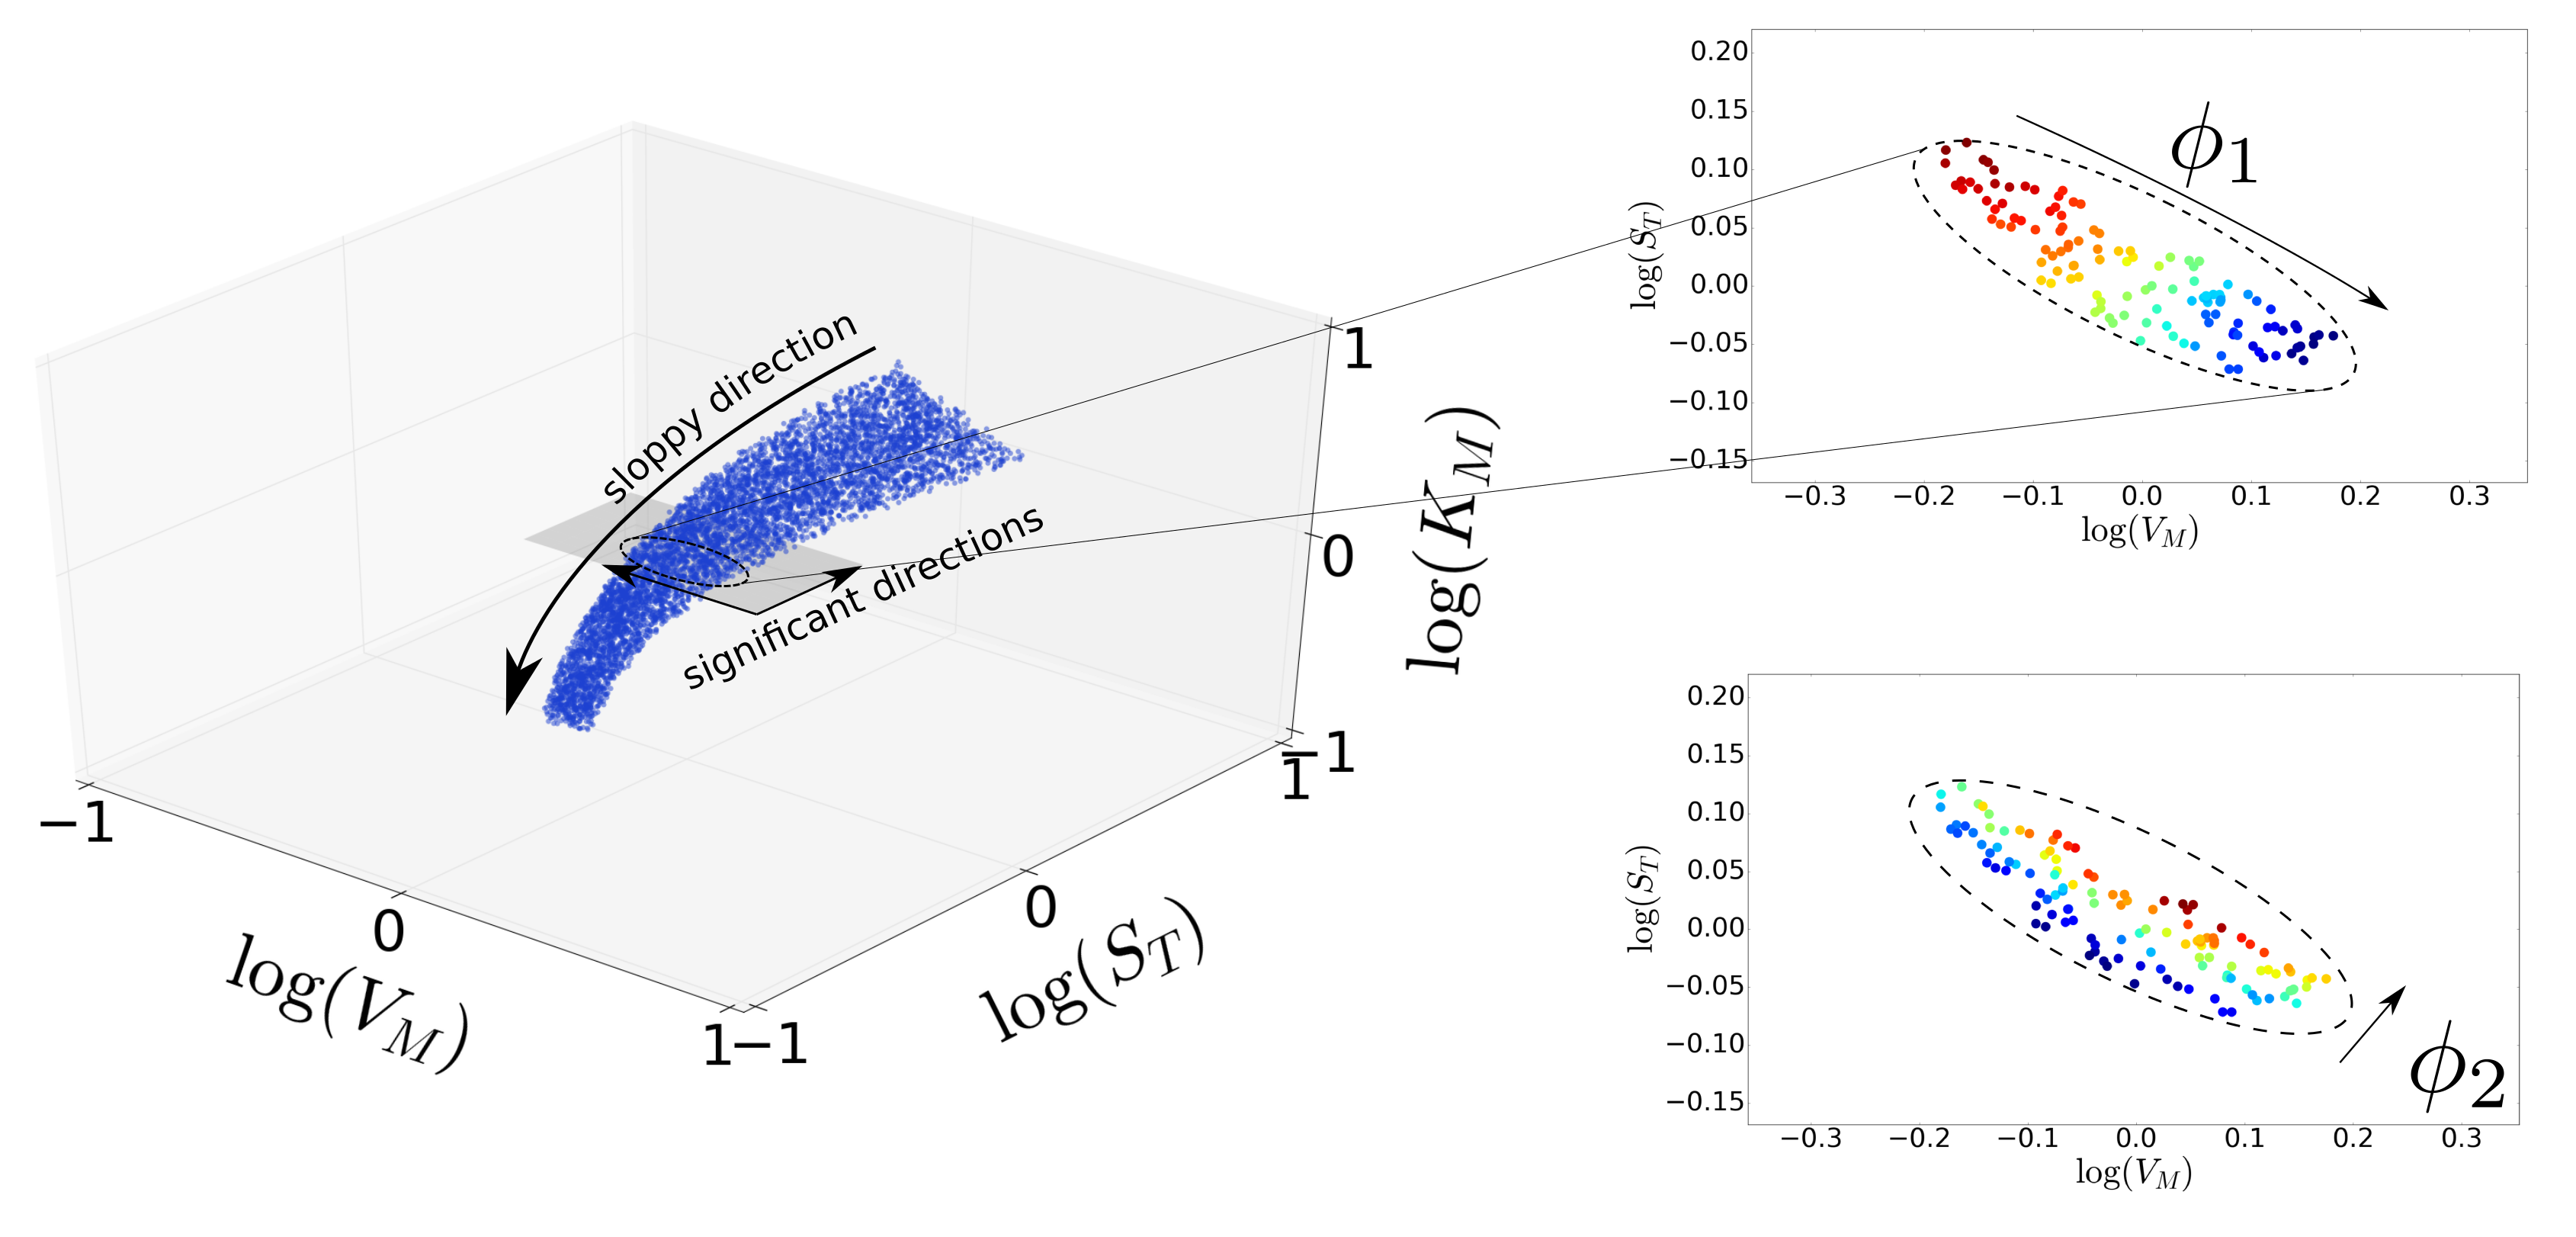
\includegraphics[width=\textwidth]{vm-st-km-all}
  \caption[DMAPS results for Michaelis-Menten system II]{(left) Scatter-plot of points in parameter space such that
    $\|f(\theta) - f^*\| < \delta$. This reveals a sloppy direction
    corresponding to the long, curved axis, and two significant
    directions orthogonal to it. (right) Two-dimensional cross section
    colored by $\phi_1$ and $\phi_2$. As expected, these eigenvectors
    do parameterize the significant directions in parameter space.
    \label{fig:mm-all} }
\end{figure}

\begin{figure}
  \centering
  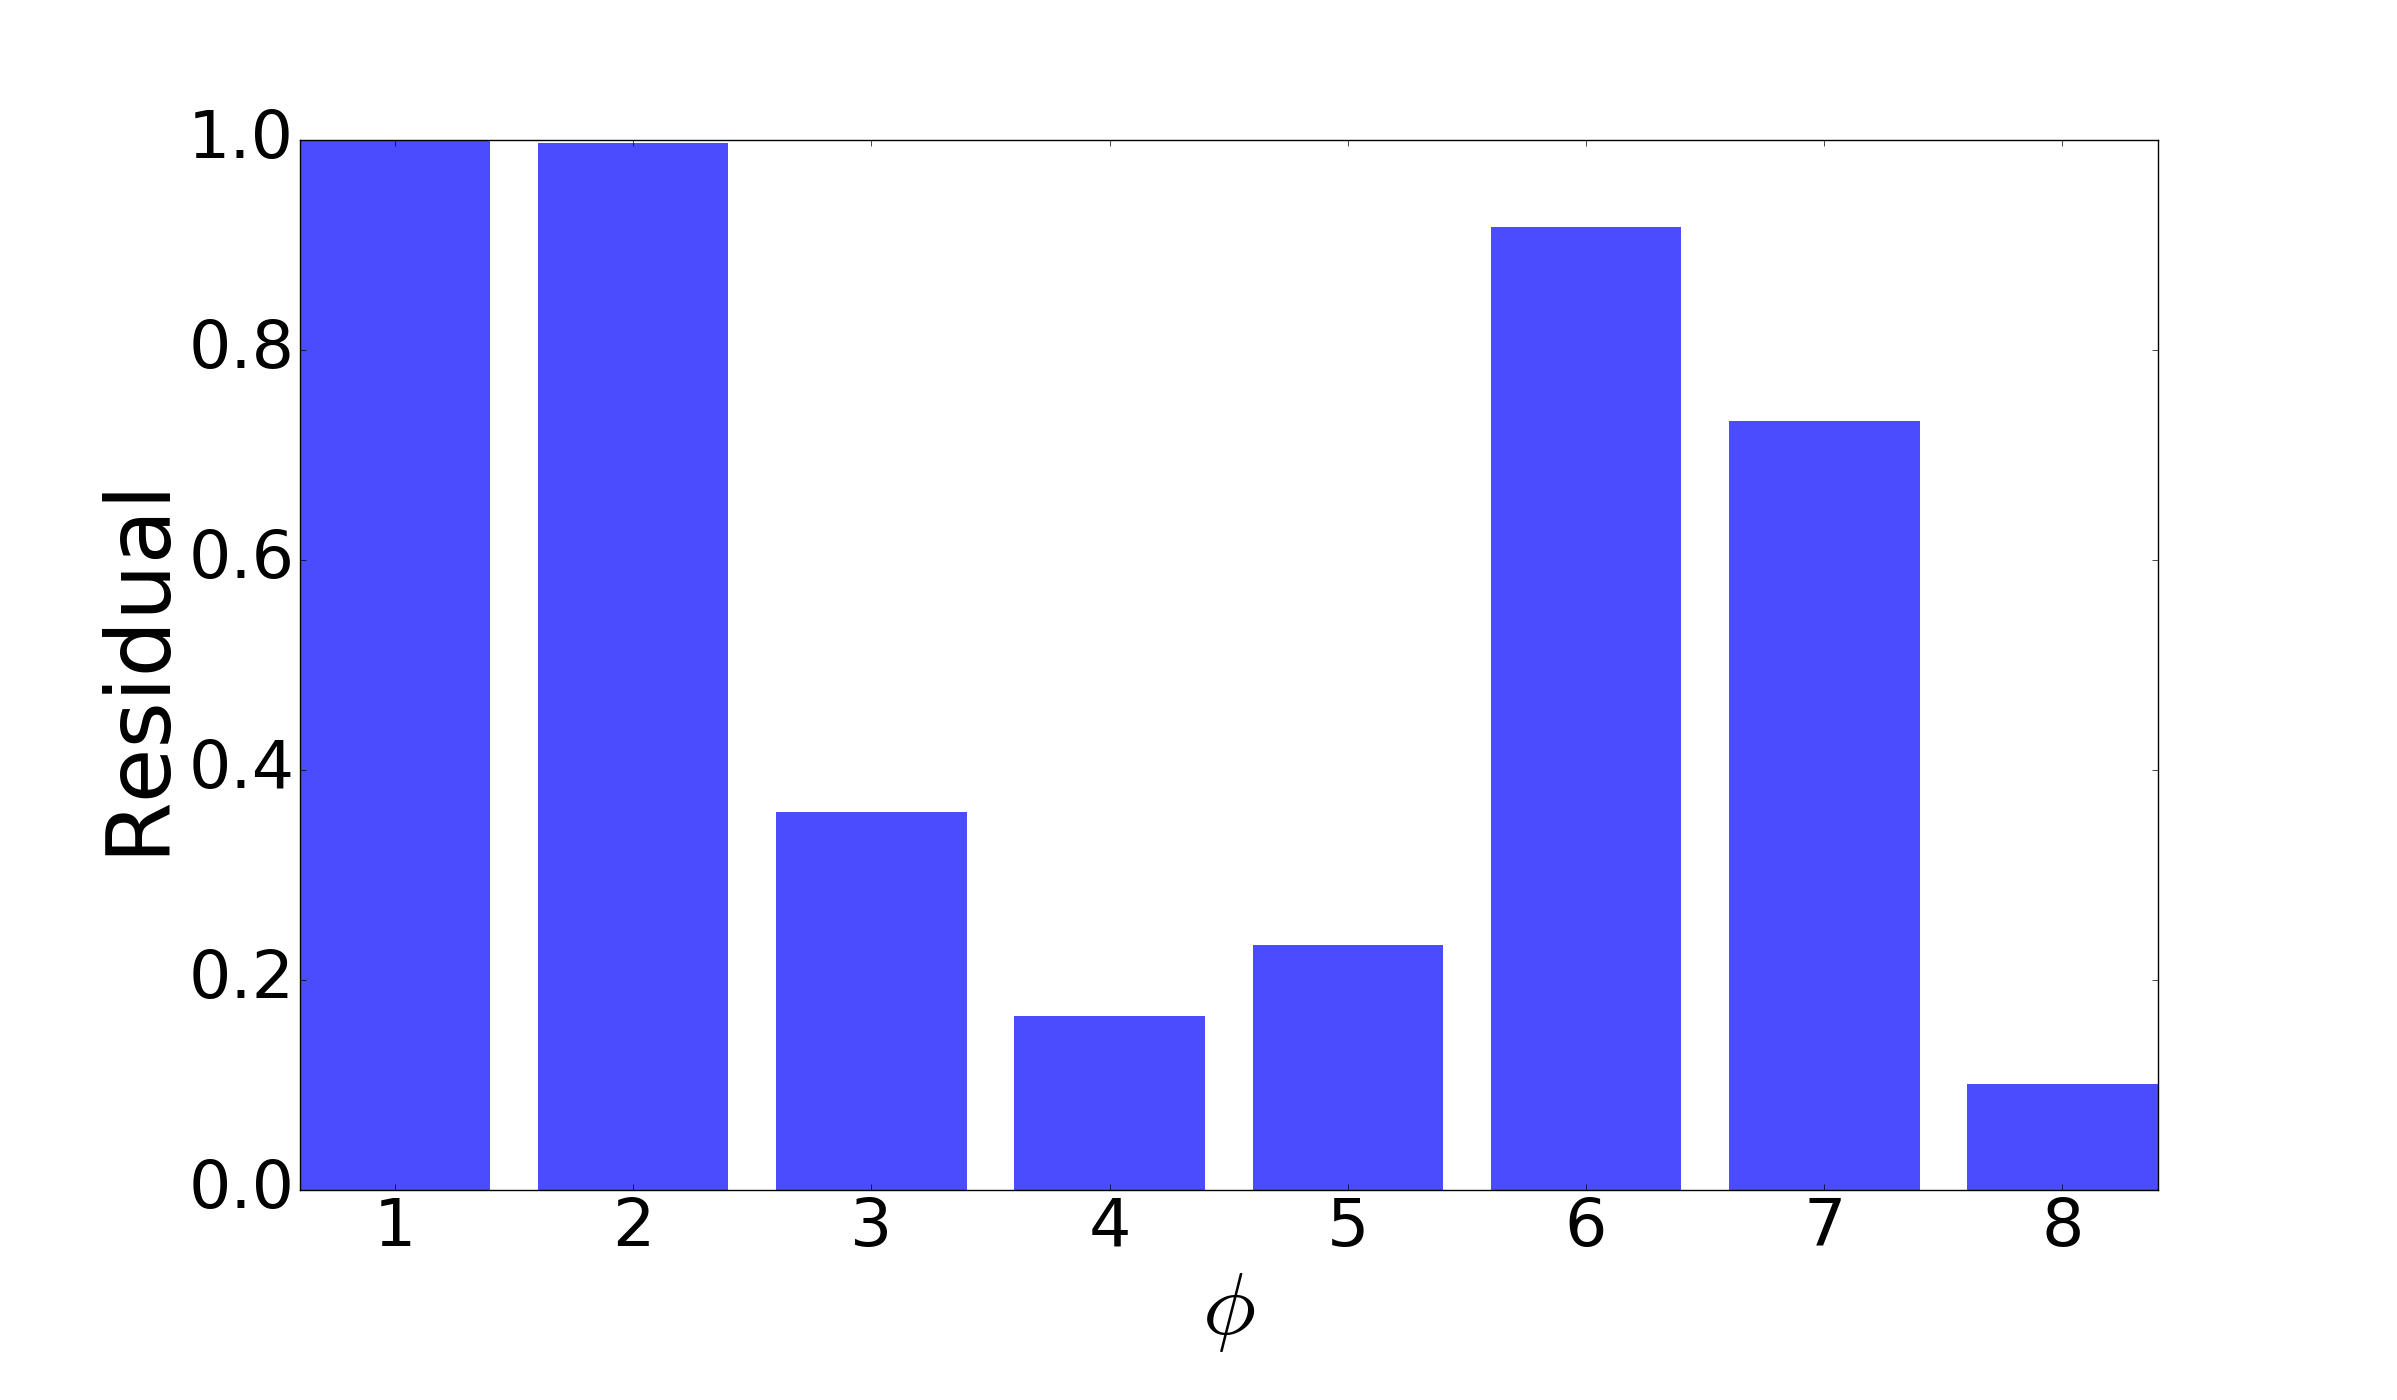
\includegraphics[width=0.6\linewidth]{residuals}
  \caption[DMAPS residuals from Michaelis-Menten system]{Residuals computed as described in previous section. High
    residuals for a given eigenvector suggest that it is not a
    function of previous eigenvectors, and thus contains new
    information. This plot suggests five significant eigenvectors, the
    first two of which parameterize significant parameter directions,
    while the final three capture sloppy
    directions. \label{fig:resids} }
\end{figure}

\section{Discussion}

The examples presented throughout this chapter show that DMAPS
consistently provides a good parameterization of the model of
interest. This parameterization is often more useful than the natural
parameter combinations originally used to formulate the system, as
DMAPS automatically accounts for regions of singular- and
regular-perturbation, in addition to detecting hidden effective
parameters. This opens the door to a number of applications, while
also inviting further research to improve certain aspects of the
method.

As we discussed in the introduction, one of the hallmarks of
sloppiness is slow convergence of model-fitting routines
\cite{transtrum_geometry_2011}. The algorithms become trapped in
sloppy regions of parameter space in which model response is nearly
constant. Thus, an obvious use of our technique would be to accelerate
these fitting procedures. The idea would be to take steps in the
DMAPS-embedding space instead of along the natural parameters. This
would require an ability to sample patches of the model manifold on
demand, and to perform extrapolation in DMAPS space. Thankfully,
results along these directions have already been established, and
these could likely be adapted to this particular setting
\cite{chiavazzo_intrinsic_2017}. We would also need the ability to map
DMAPS coordinates back to points on the model manifold. This is
related to the problem of ``lifting'' in the Equation Free framework,
again an area where existing work may be quickly incorporated
\cite{rajendran_data_2016,laing_equation-free_2015,laing_coarse-grained_2007}.

Another avenue would be nonlinear sensitivity analysis. The
simplest and most common methods simply vary individual parameters
while observing changes in model output
\cite{murphy_quantification_2004}. The shortcomings of such studies
are well known \cite{saltelli_how_2010},
but even more sophisticated methods designed for nonlinear models
assume that each parameter can be treated independently of the
others \cite{cukier_nonlinear_1978}. It would clearly be useful to
adapt this technique to the task. A simple start would be to assess
how many significant parameters a system has based on the dimension of
the DMAPS embedding \cite{dsilva_parsimonious_2015}.

Finally, further work is needed to accelerate sampling on the model
manifold. The current approach, approximate Bayesian computation, is
simple to implement but scales poorly with the dimension of parameter
space, $k$ \cite{turner_tutorial_2012}. One possibility would be to
calculate the convex hull or alpha-shape of a small sample, and then
interpolate among these points
\cite{barber_quickhull_1996,edelsbrunner_three-dimensional_1994}. Overall,
this chapter presents a novel, data-driven method to parameterize
complex models that will hopefully form the foundation for future,
practical applications.


%%% Local Variables: ***
%%% mode:latex ***
%%% TeX-master: "../../thesis.tex"  ***
%%% End: ***
